% !TeX root = ../tfg.tex
% !TeX encoding = utf8

\chapter{Material complementario}\label{ap:complementario}

\section{Explicaciones por ejemplos de STOOD-X}\label{sec:apc-stoodx}

% Complementa la \cref{sec:stoodx-ejemplos}. En cada figura, la primera columna es la imagen evaluada y
% las cinco siguientes, sus vecinos de entrenamiento, con la clase predicha, la puntuación (p y z)
% y las distancias en los títulos. Selección: entre el 10 % con -z más alto o más bajo, 5 al azar
% con semilla 0 (RESUMEN_STOODX.md).
\pendiente{presentación de las figuras}

\subsection{Con $K = 500$}\label{sec:apc-k500}

\begin{figure}[tbp]
  \centering
  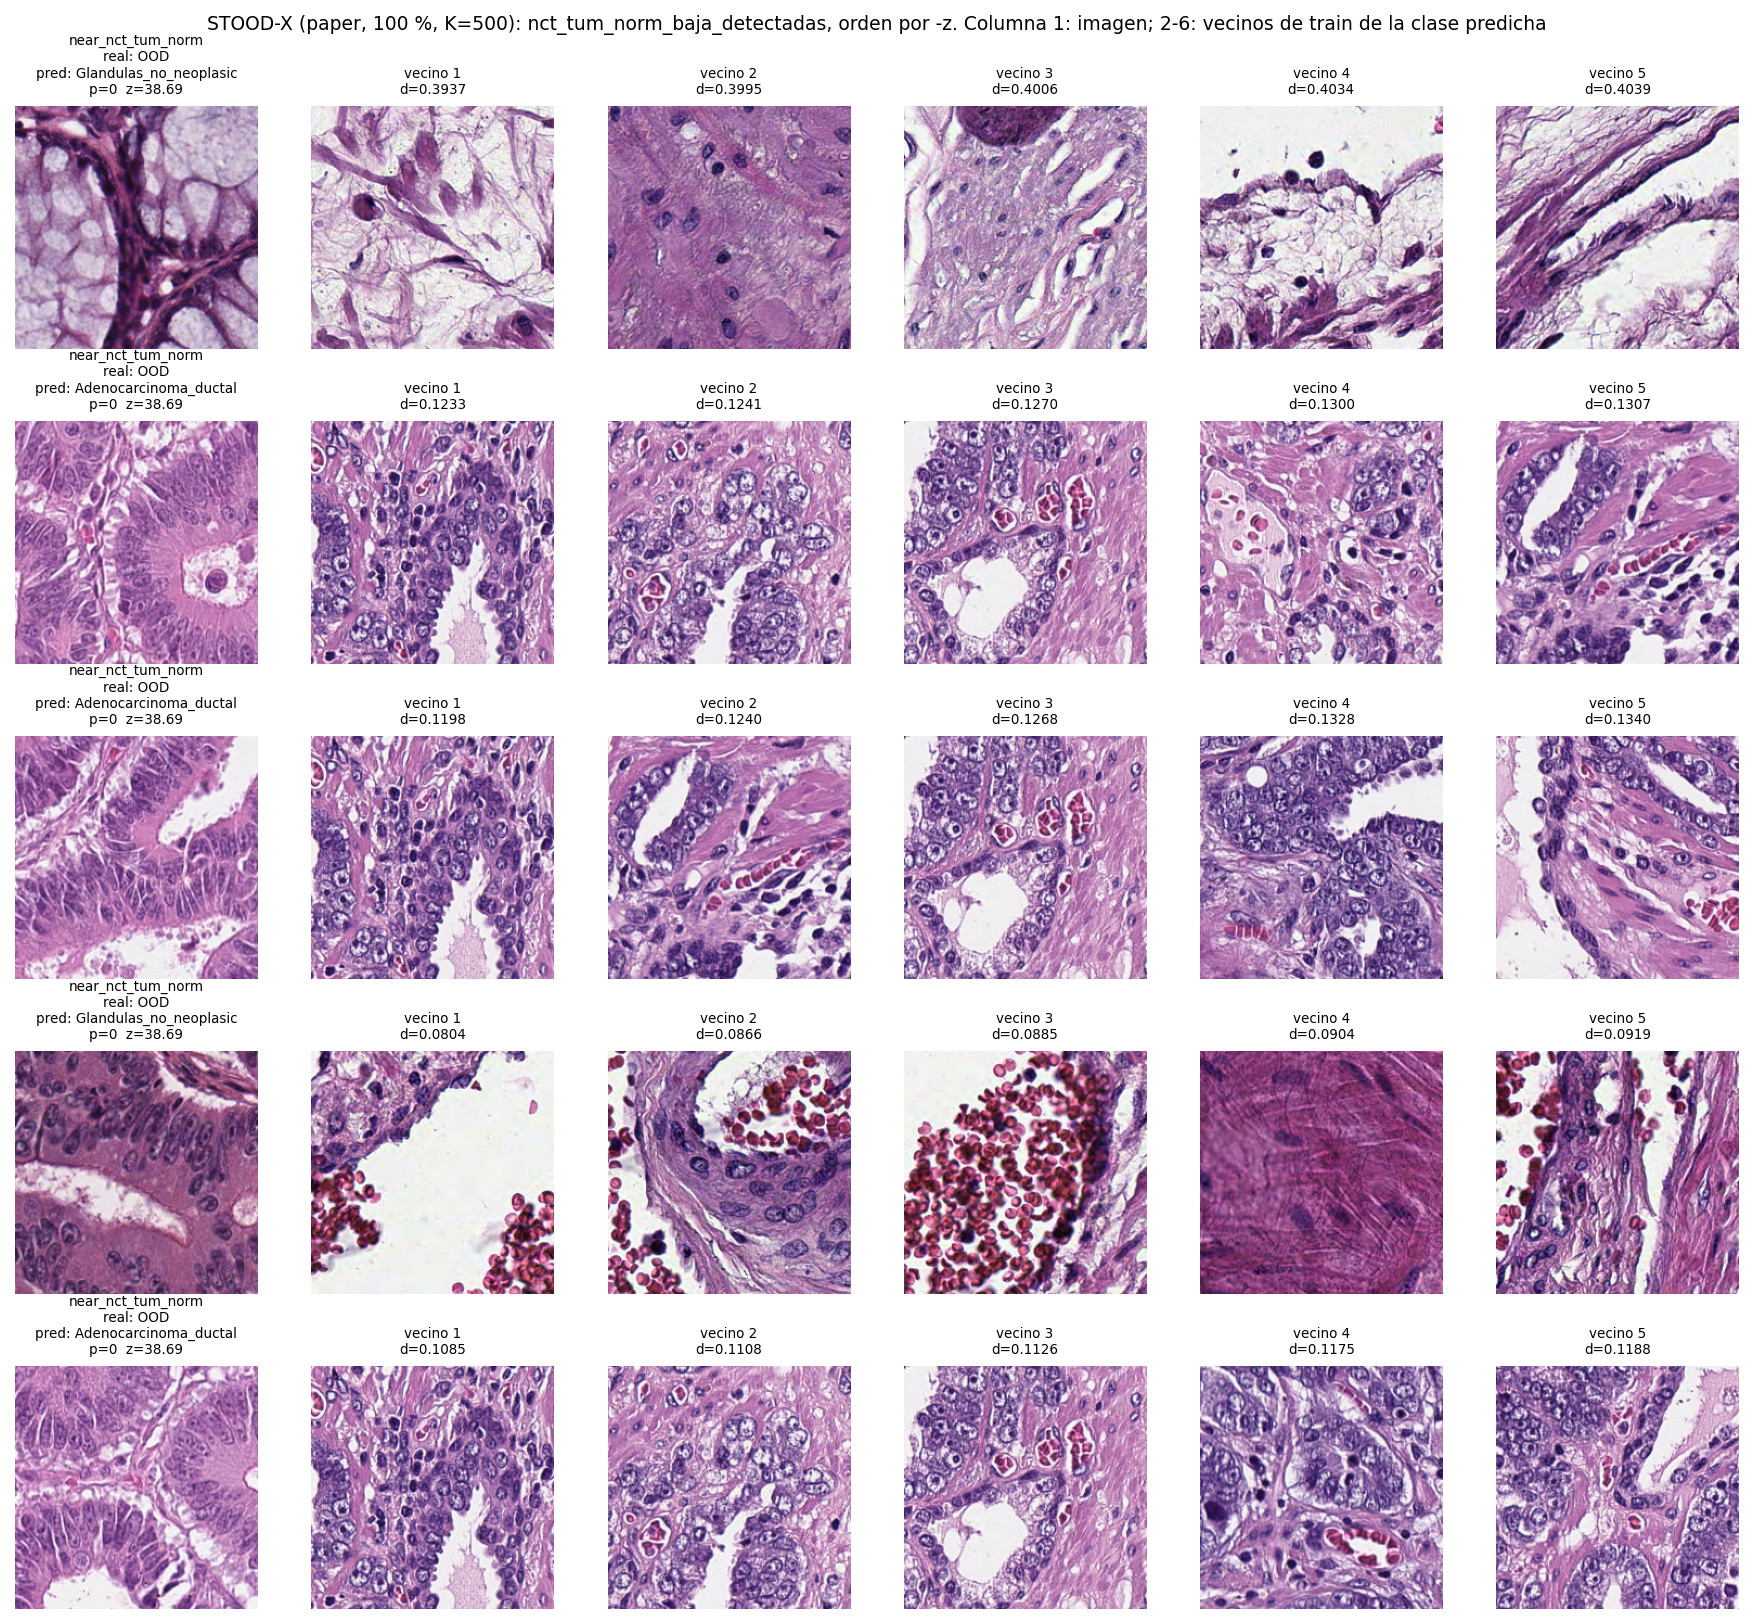
\includegraphics[width=\textwidth]{img/apC/ejemplos_K500_nct_tum_norm_baja_detectadas.jpg}
  \caption{STOOD-X ($K = 500$): cinco imágenes de TUM+NORM bien detectadas como OOD y sus vecinos de entrenamiento de la clase predicha.}
  \label{fig:stoodx-ejemplos-detectadas}
\end{figure}

\begin{figure}[tbp]
  \centering
  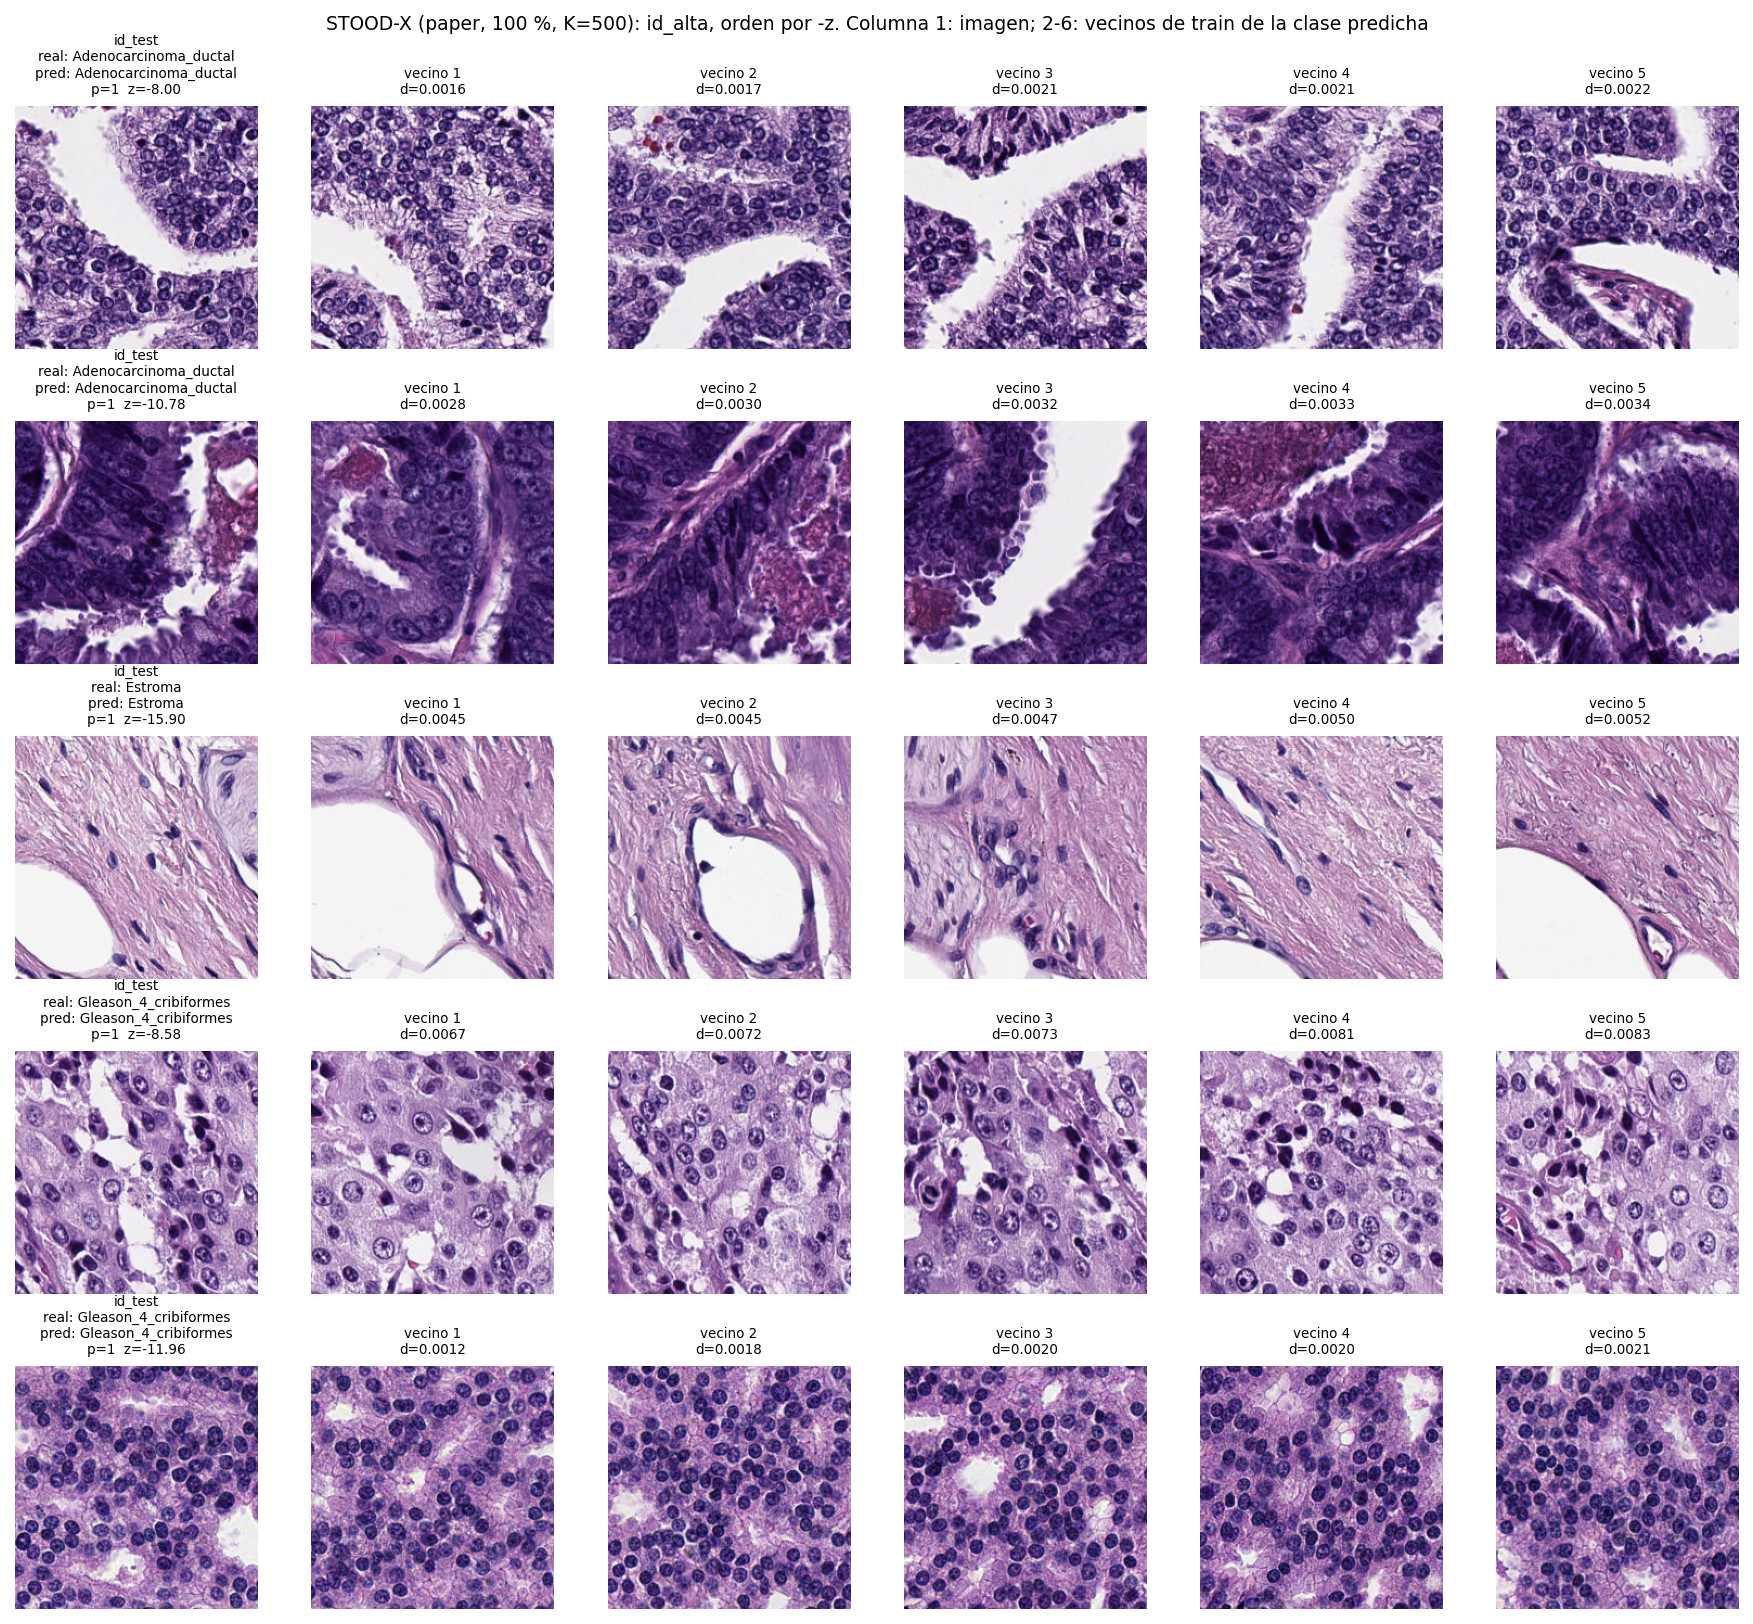
\includegraphics[width=\textwidth]{img/apC/ejemplos_K500_id_alta.jpg}
  \caption{STOOD-X ($K = 500$): cinco imágenes ID con puntuación alta y sus vecinos de entrenamiento de la clase predicha: casos ID típicos.}
  \label{fig:stoodx-ejemplos-id}
\end{figure}

\begin{figure}[tbp]
  \centering
  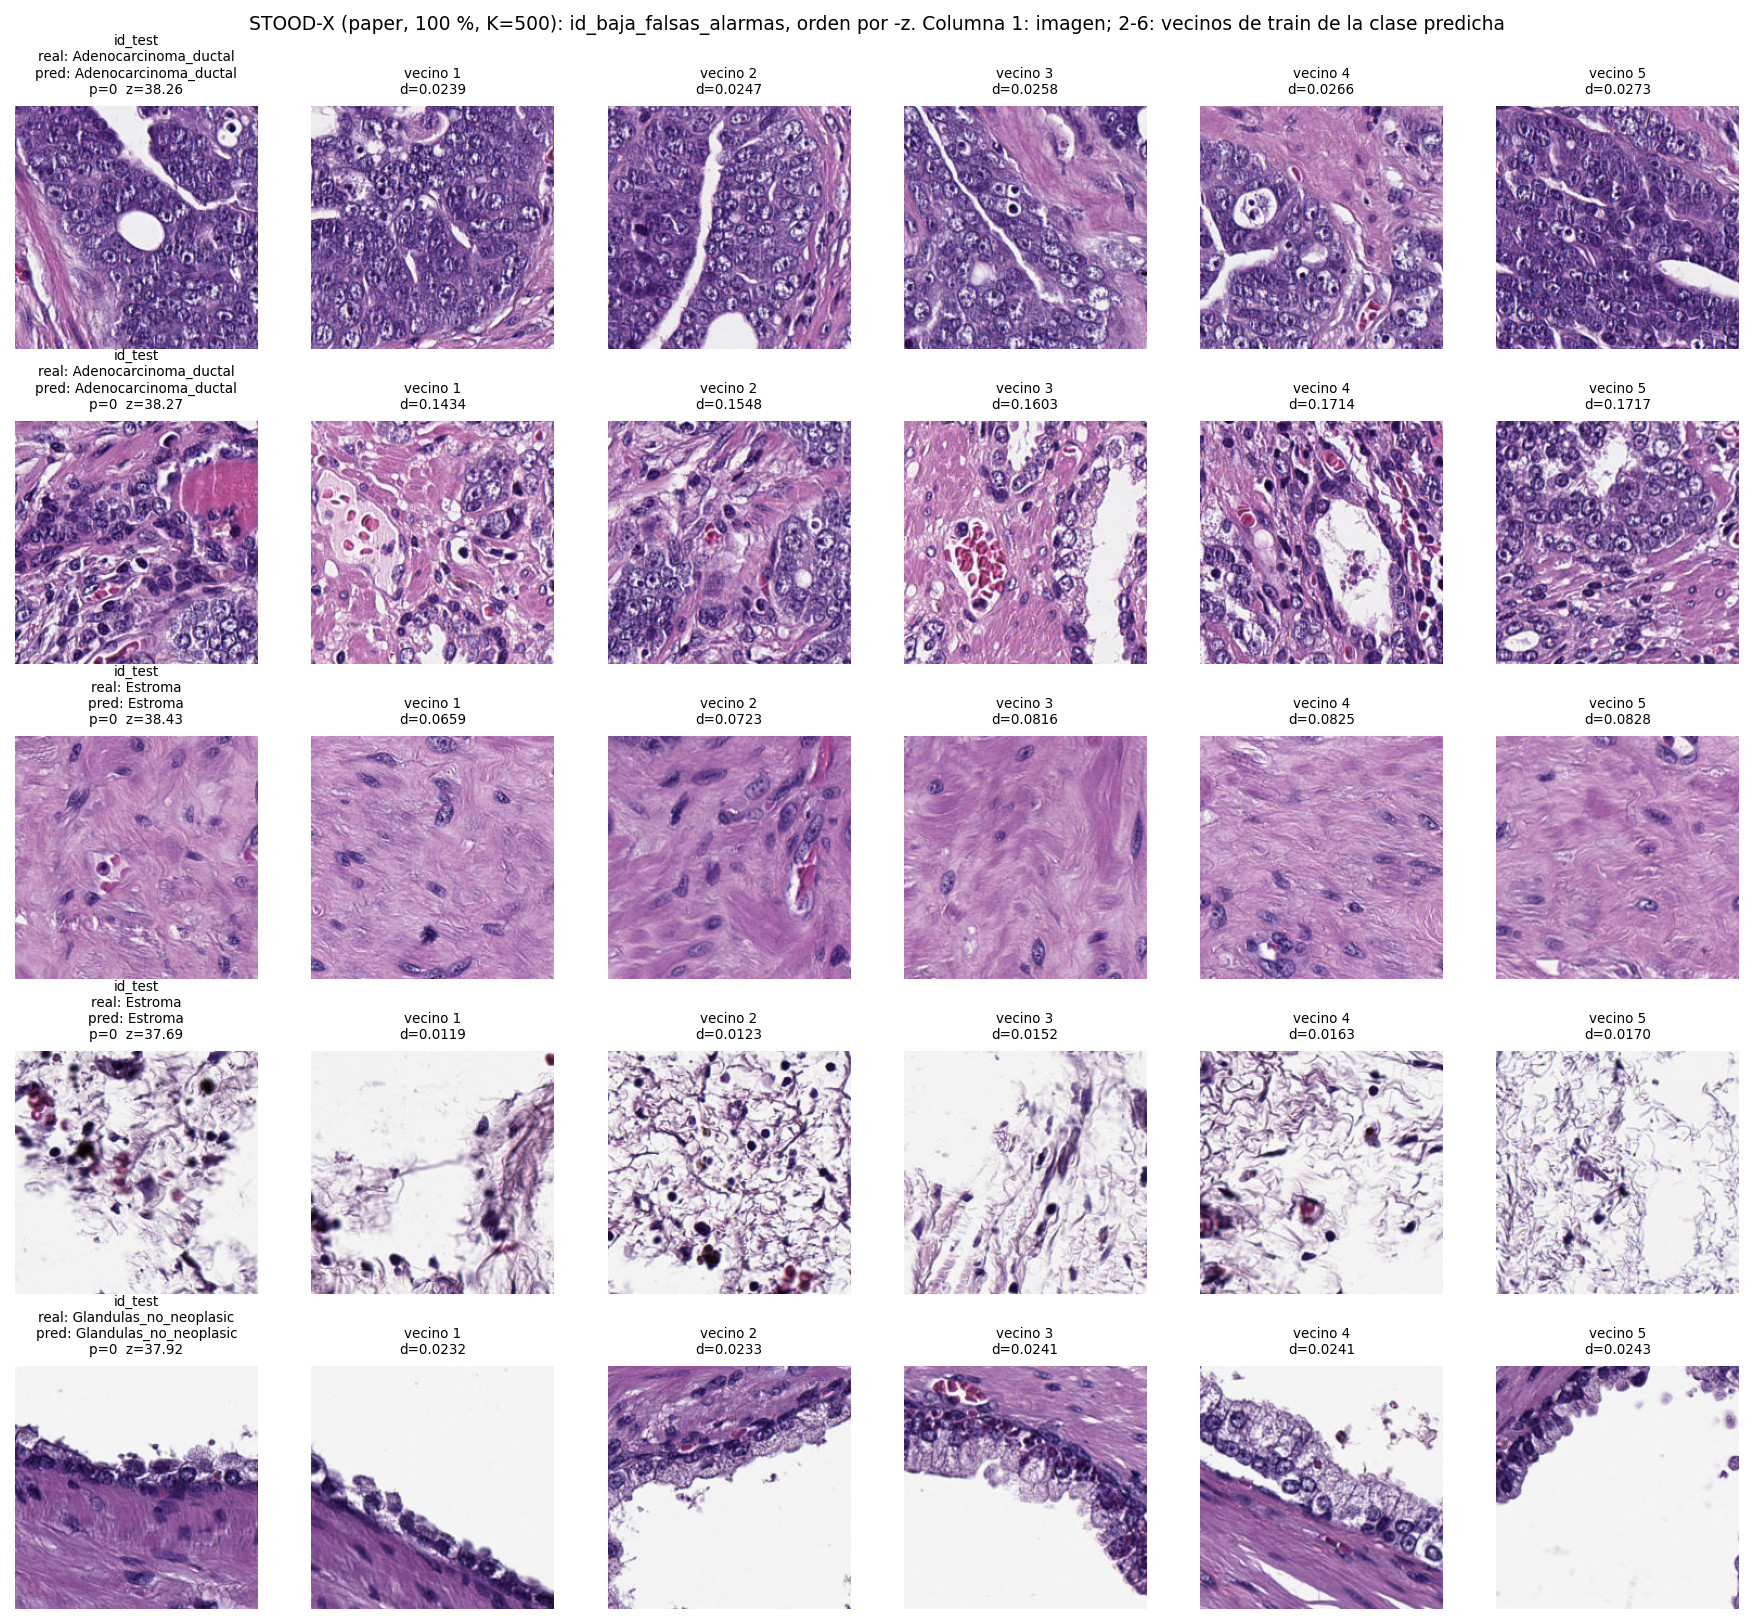
\includegraphics[width=\textwidth]{img/apC/ejemplos_K500_id_baja_falsas_alarmas.jpg}
  \caption{STOOD-X ($K = 500$): cinco imágenes ID con puntuación baja (falsas alarmas) y sus vecinos de entrenamiento ($z$ saturada, $\approx 38$).}
  \label{fig:stoodx-ejemplos-falsas}
\end{figure}

\begin{figure}[tbp]
  \centering
  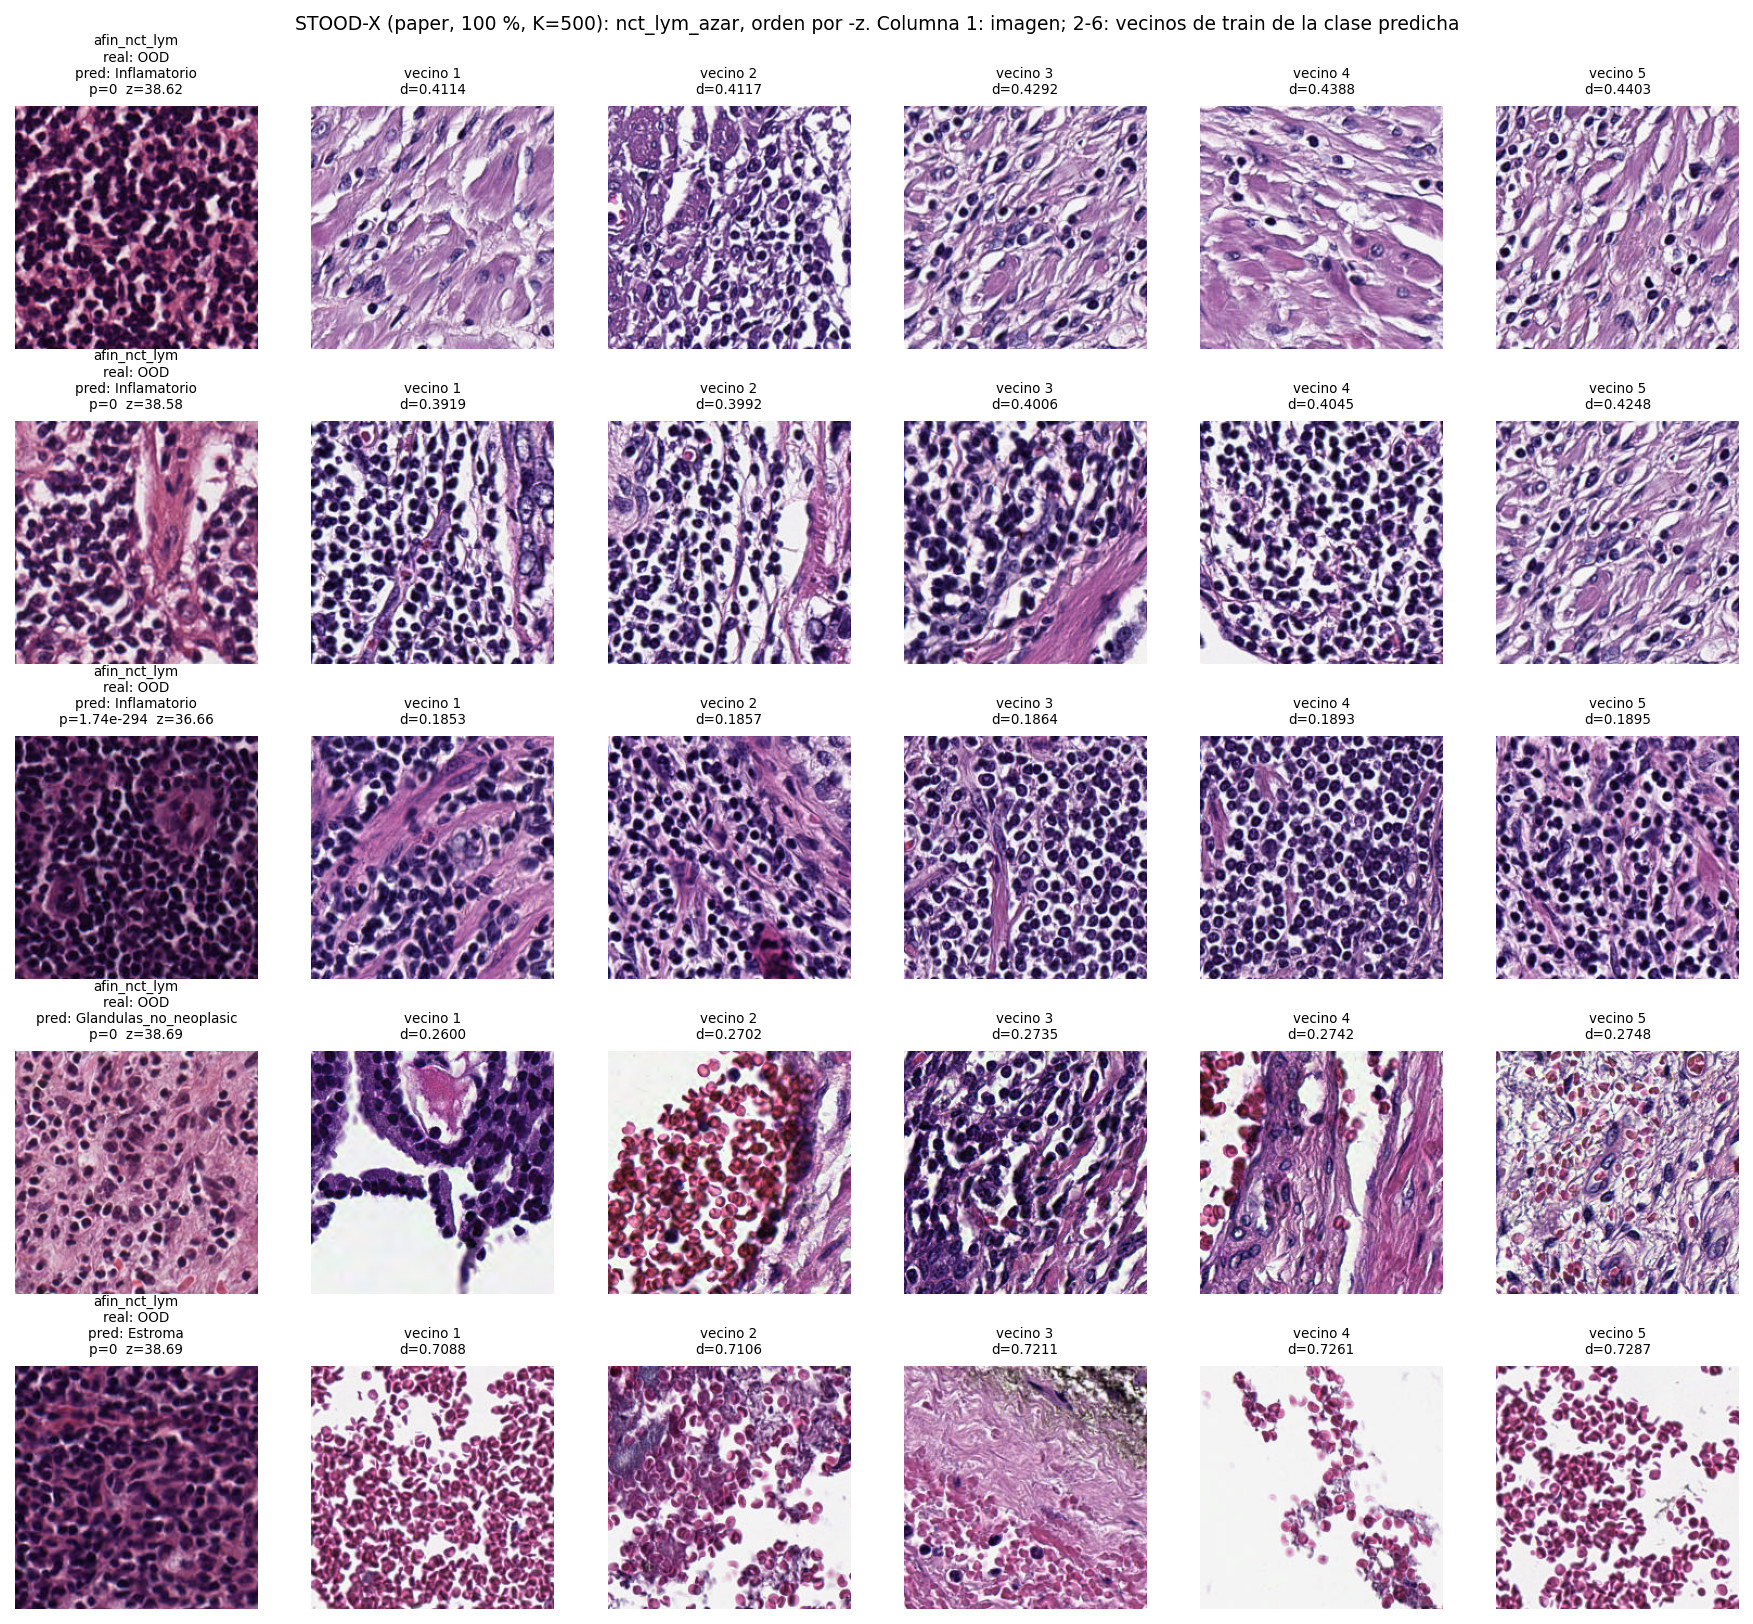
\includegraphics[width=\textwidth]{img/apC/ejemplos_K500_nct_lym_azar.jpg}
  \caption{STOOD-X ($K = 500$): cinco imágenes de LYM elegidas al azar y sus vecinos de entrenamiento de la clase predicha.}
  \label{fig:stoodx-ejemplos-lym}
\end{figure}

\begin{figure}[tbp]
  \centering
  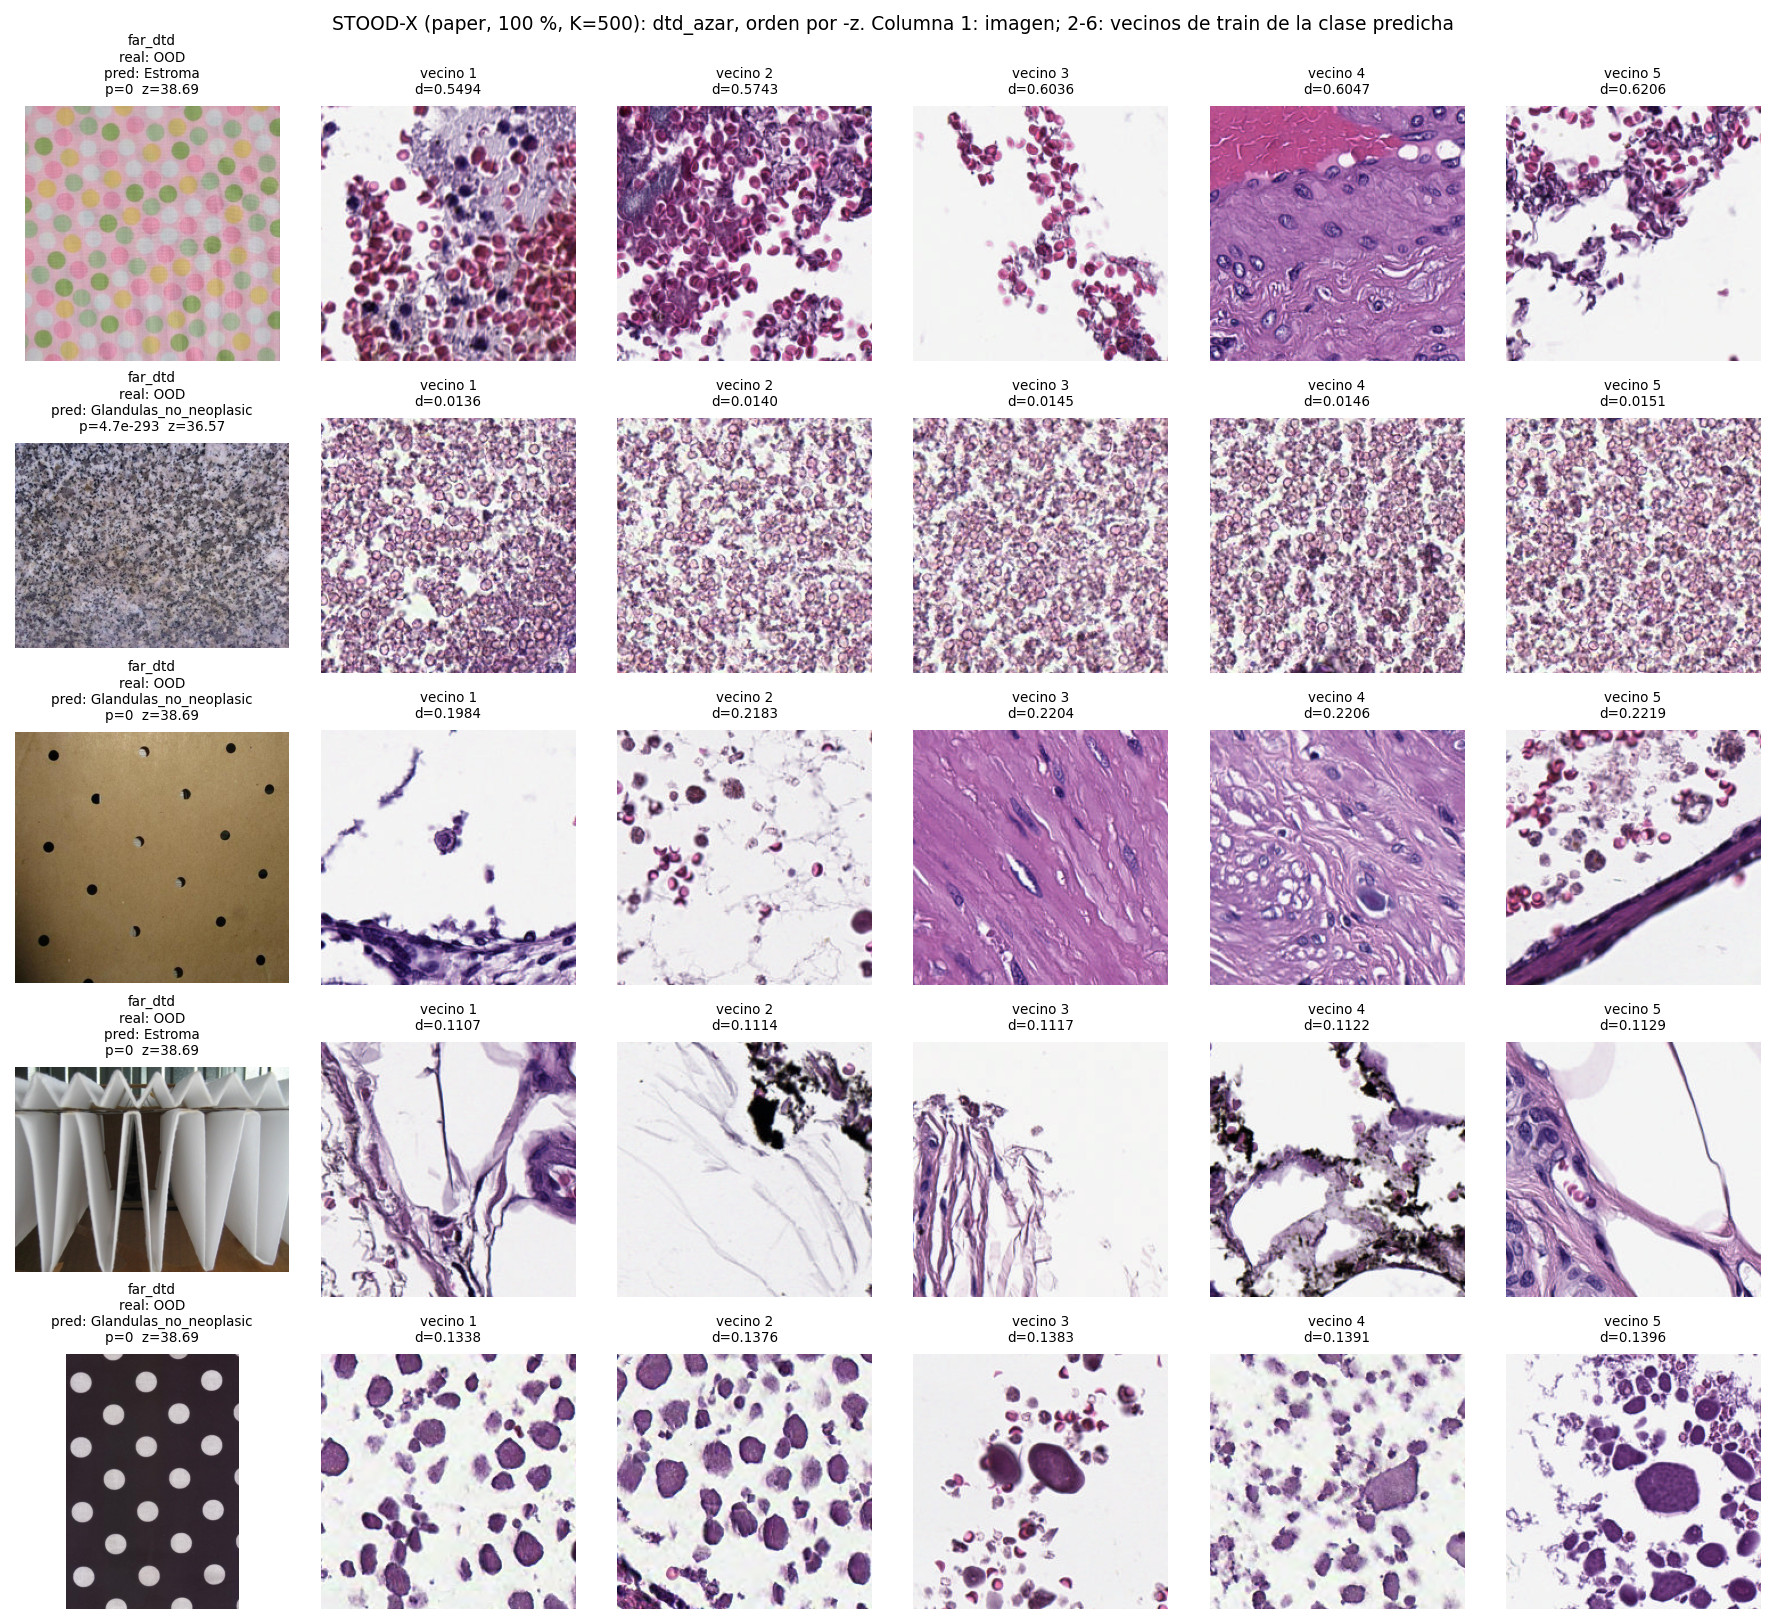
\includegraphics[width=\textwidth]{img/apC/ejemplos_K500_dtd_azar.jpg}
  \caption{STOOD-X ($K = 500$): cinco imágenes de DTD elegidas al azar y sus vecinos de entrenamiento de la clase predicha.}
  \label{fig:stoodx-ejemplos-dtd}
\end{figure}

\subsection{Con la variante exploratoria $K_c$}\label{sec:apc-kc}

% Variante exploratoria K_c = min(500, floor(n_c/2)), con resultado negativo (\cref{sec:stoodx-k}).
% Con K_c, las cinco TUM+NORM aceptadas también se predicen Gleason_5_comedonecrosis.
\pendiente{presentación de las figuras}

\begin{figure}[tbp]
  \centering
  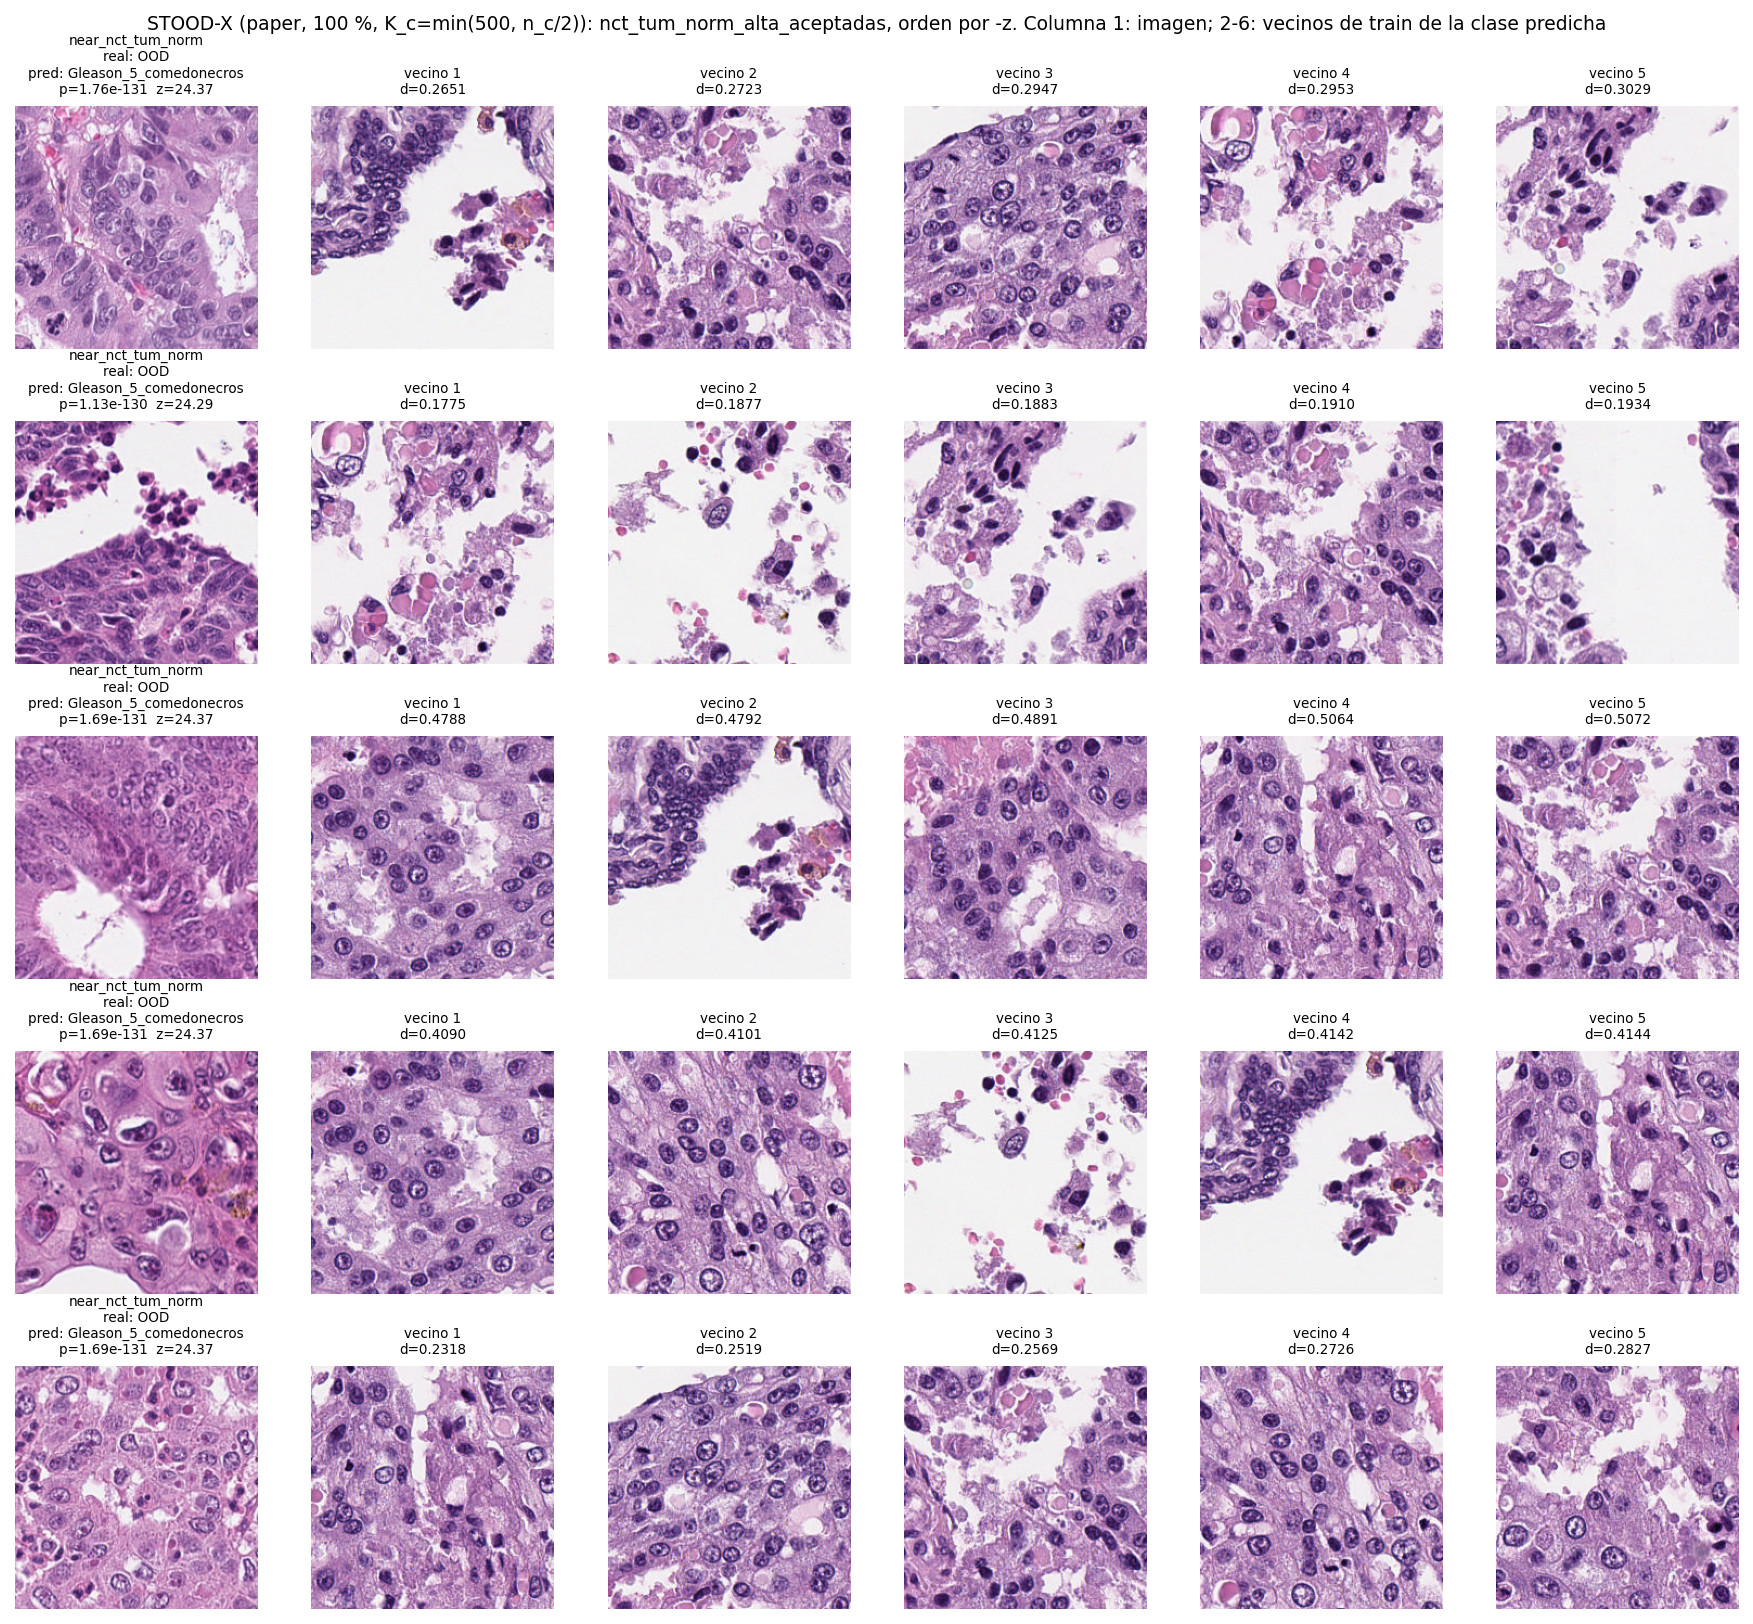
\includegraphics[width=\textwidth]{img/apC/ejemplos_kc_nct_tum_norm_alta_aceptadas.jpg}
  \caption{STOOD-X (variante exploratoria $K_c$): cinco imágenes de TUM+NORM aceptadas como ID y sus vecinos de entrenamiento de la clase predicha.}
  \label{fig:stoodx-kc-tumnorm-aceptadas}
\end{figure}

\begin{figure}[tbp]
  \centering
  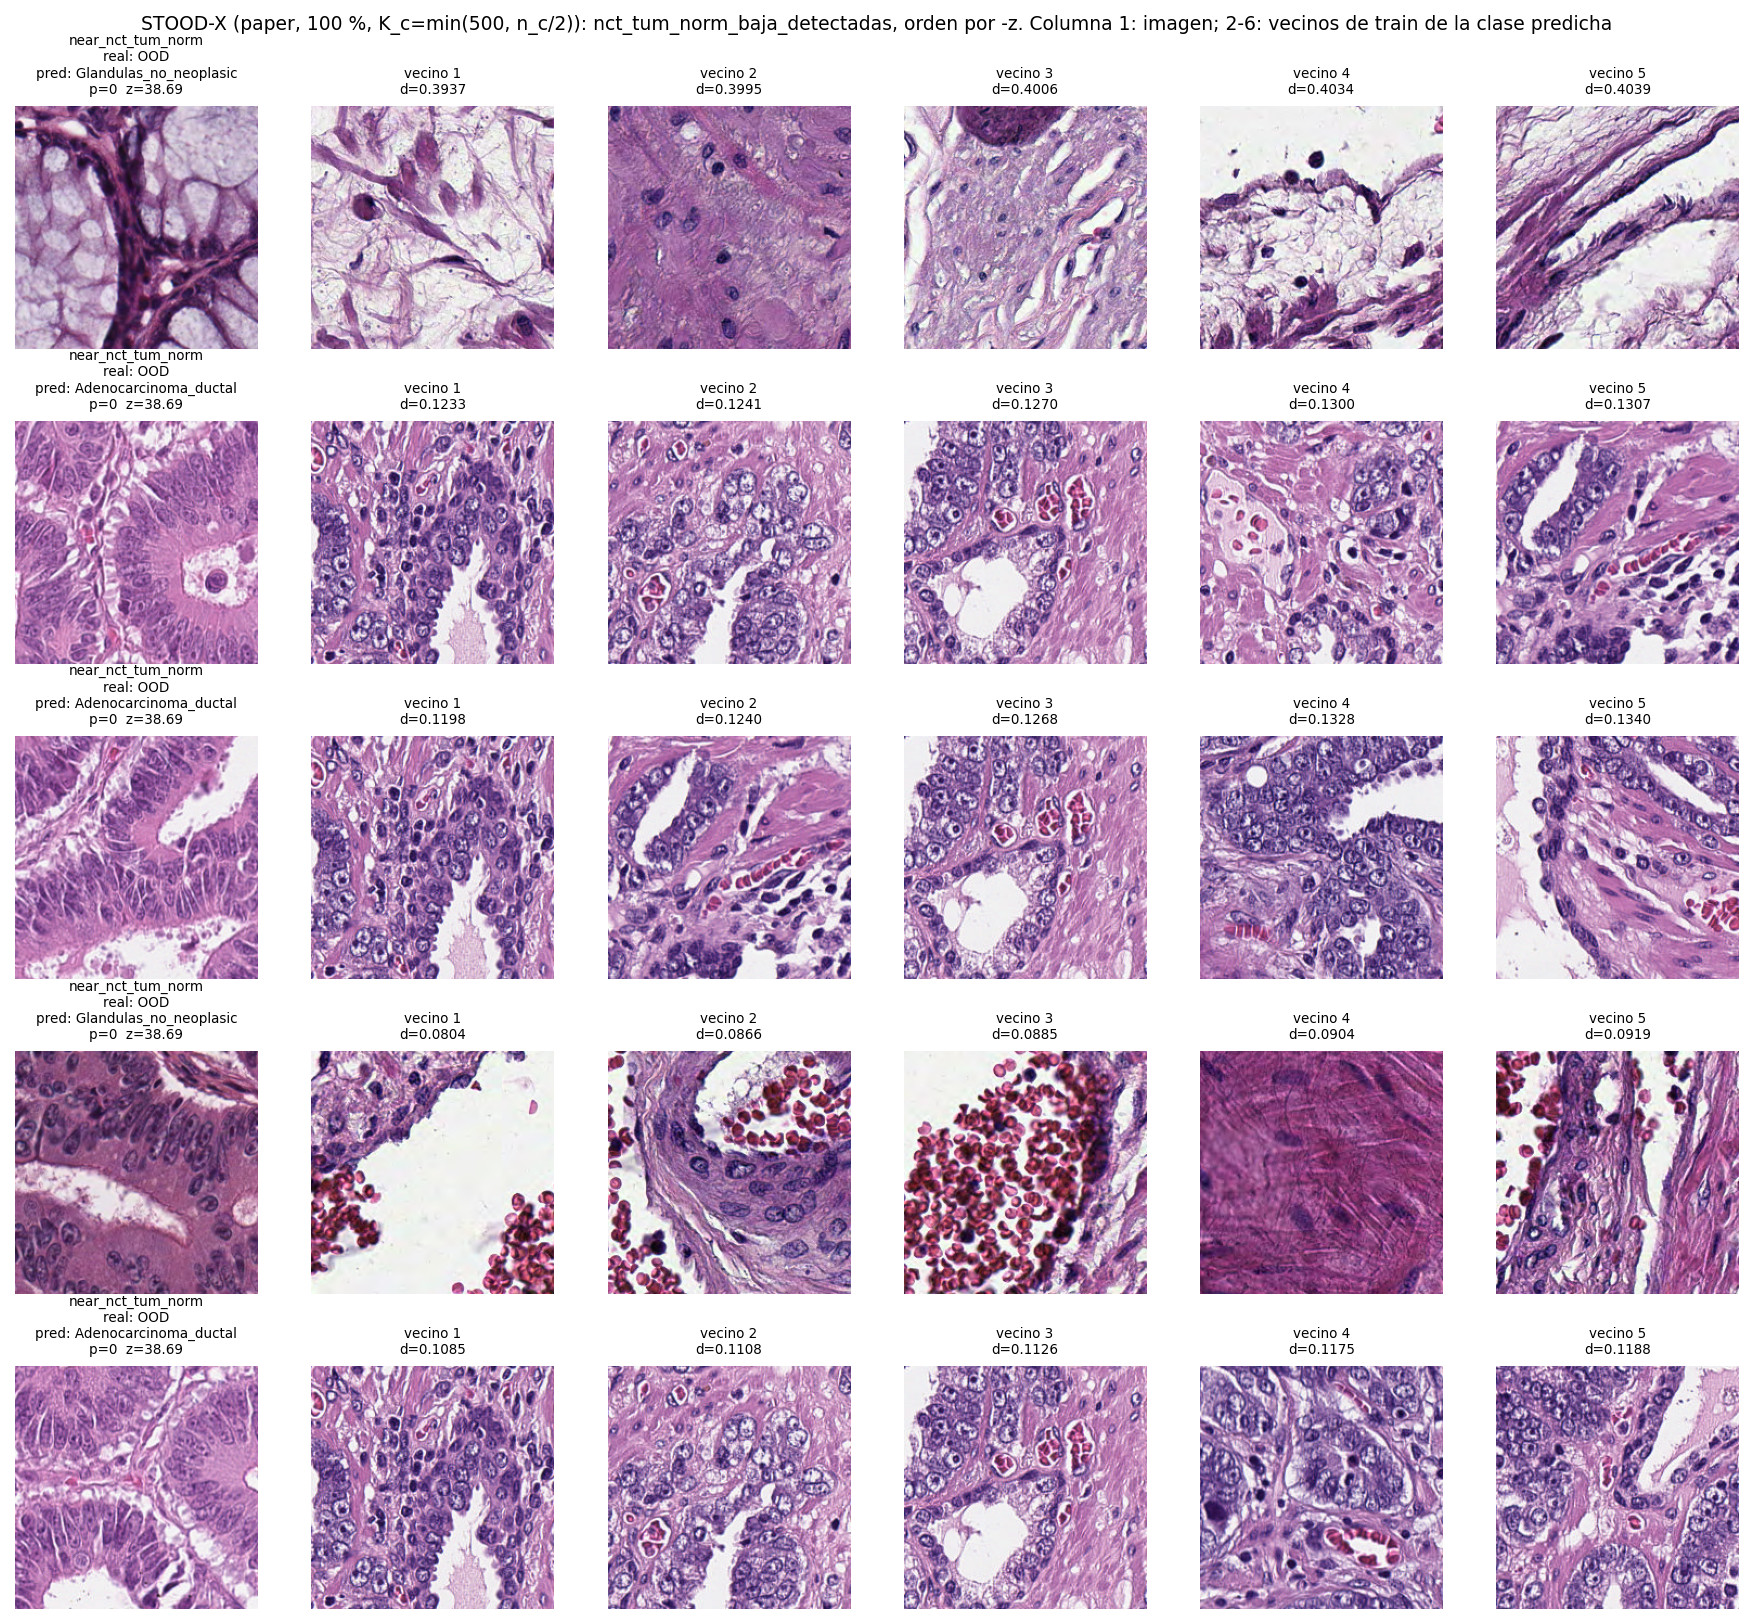
\includegraphics[width=\textwidth]{img/apC/ejemplos_kc_nct_tum_norm_baja_detectadas.jpg}
  \caption{STOOD-X (variante exploratoria $K_c$): cinco imágenes de TUM+NORM bien detectadas como OOD y sus vecinos de entrenamiento de la clase predicha.}
  \label{fig:stoodx-kc-tumnorm-detectadas}
\end{figure}

\begin{figure}[tbp]
  \centering
  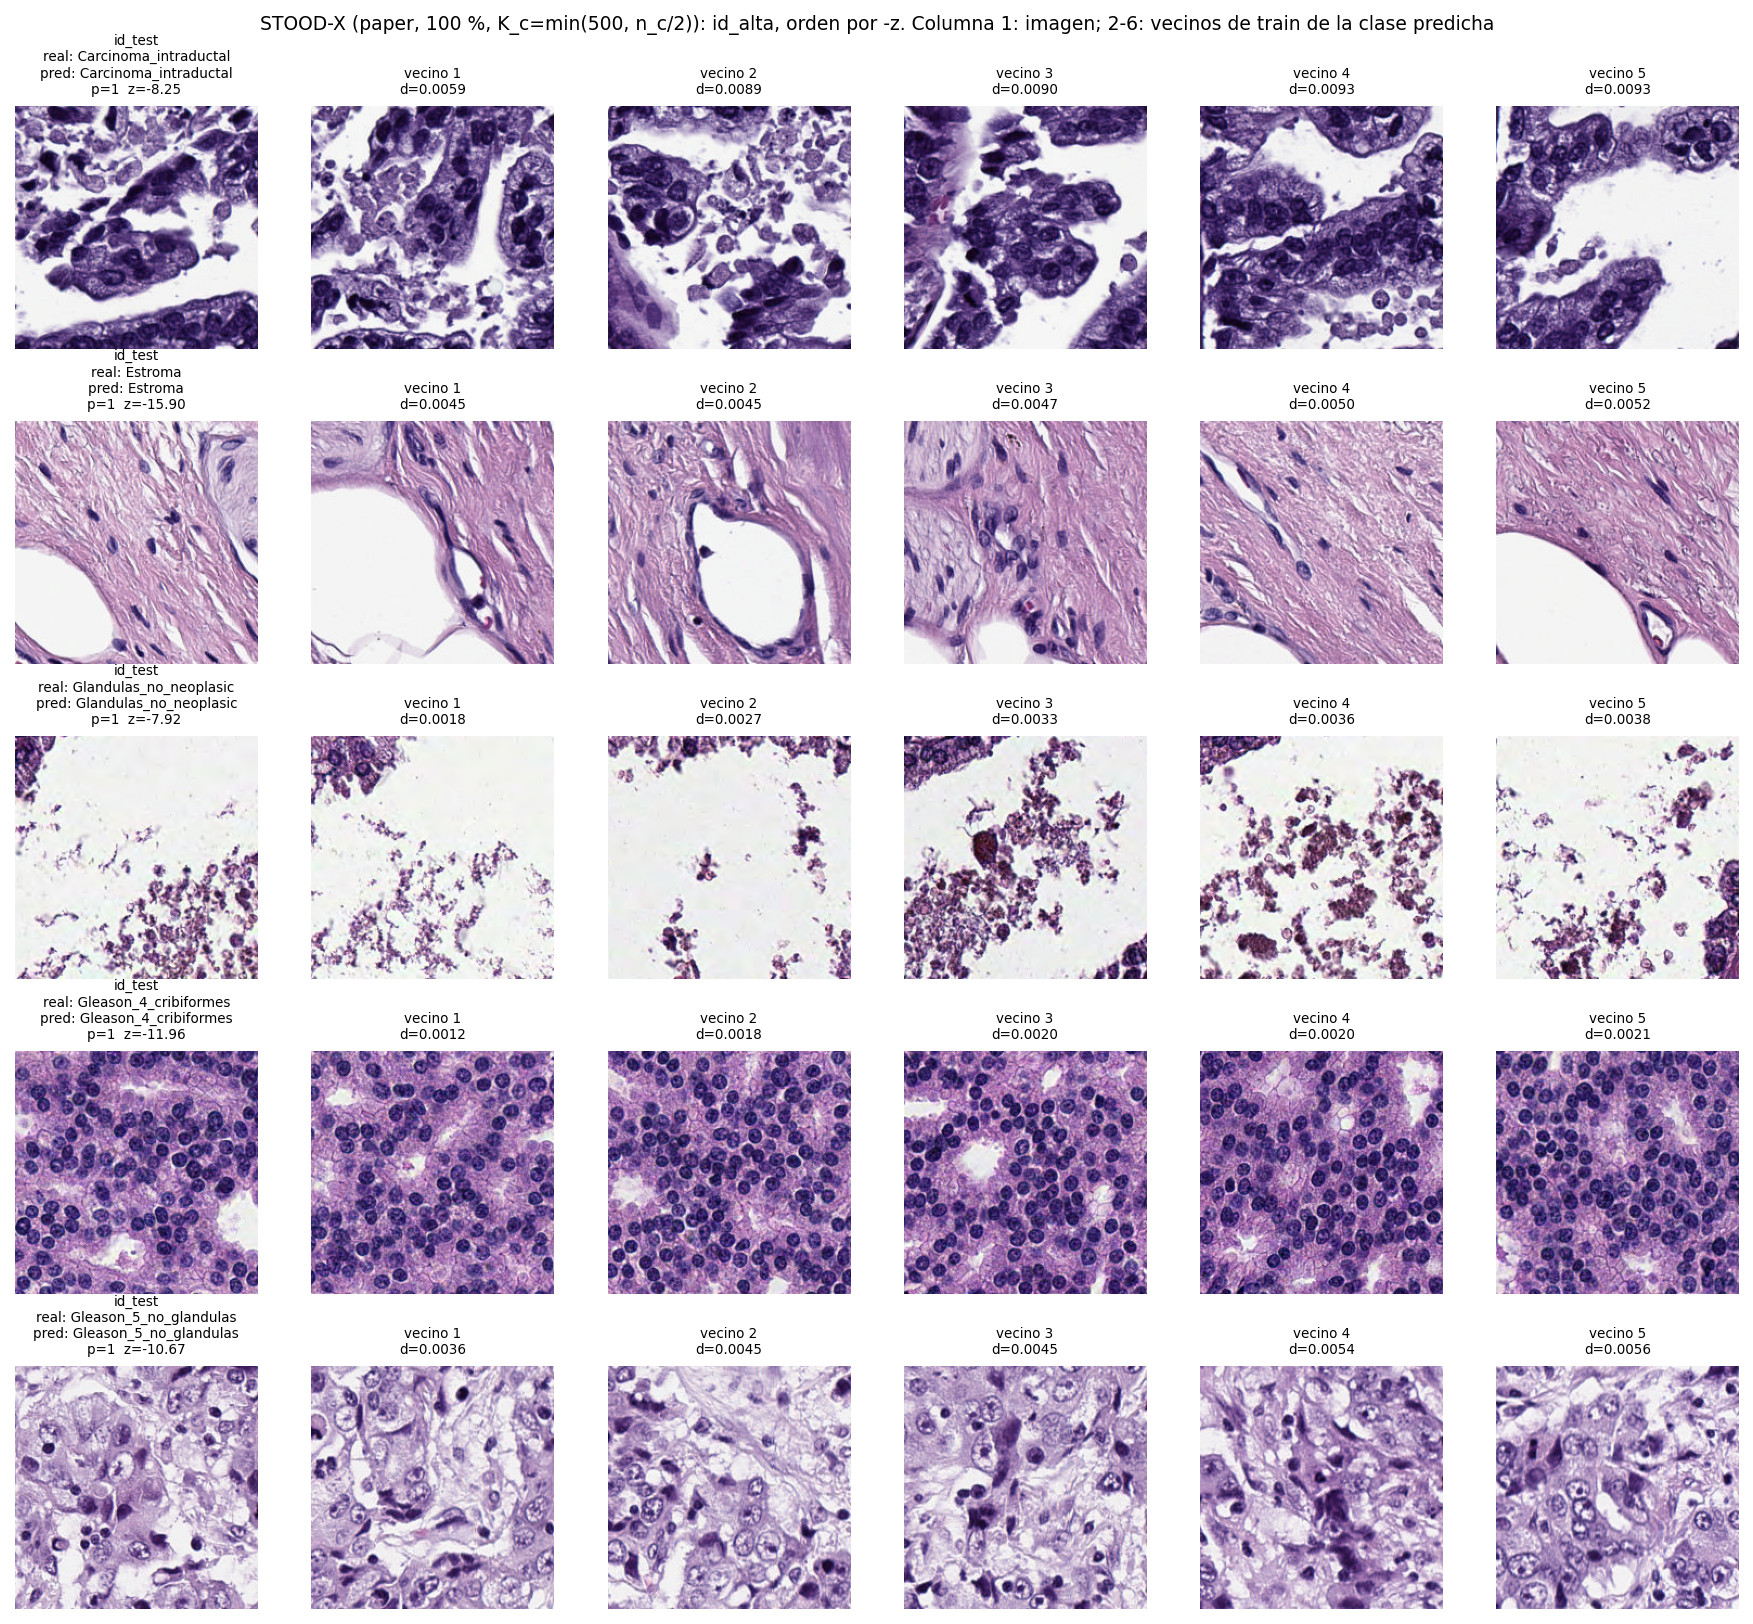
\includegraphics[width=\textwidth]{img/apC/ejemplos_kc_id_alta.jpg}
  \caption{STOOD-X (variante exploratoria $K_c$): cinco imágenes ID con puntuación alta y sus vecinos de entrenamiento de la clase predicha.}
  \label{fig:stoodx-kc-id-alta}
\end{figure}

\begin{figure}[tbp]
  \centering
  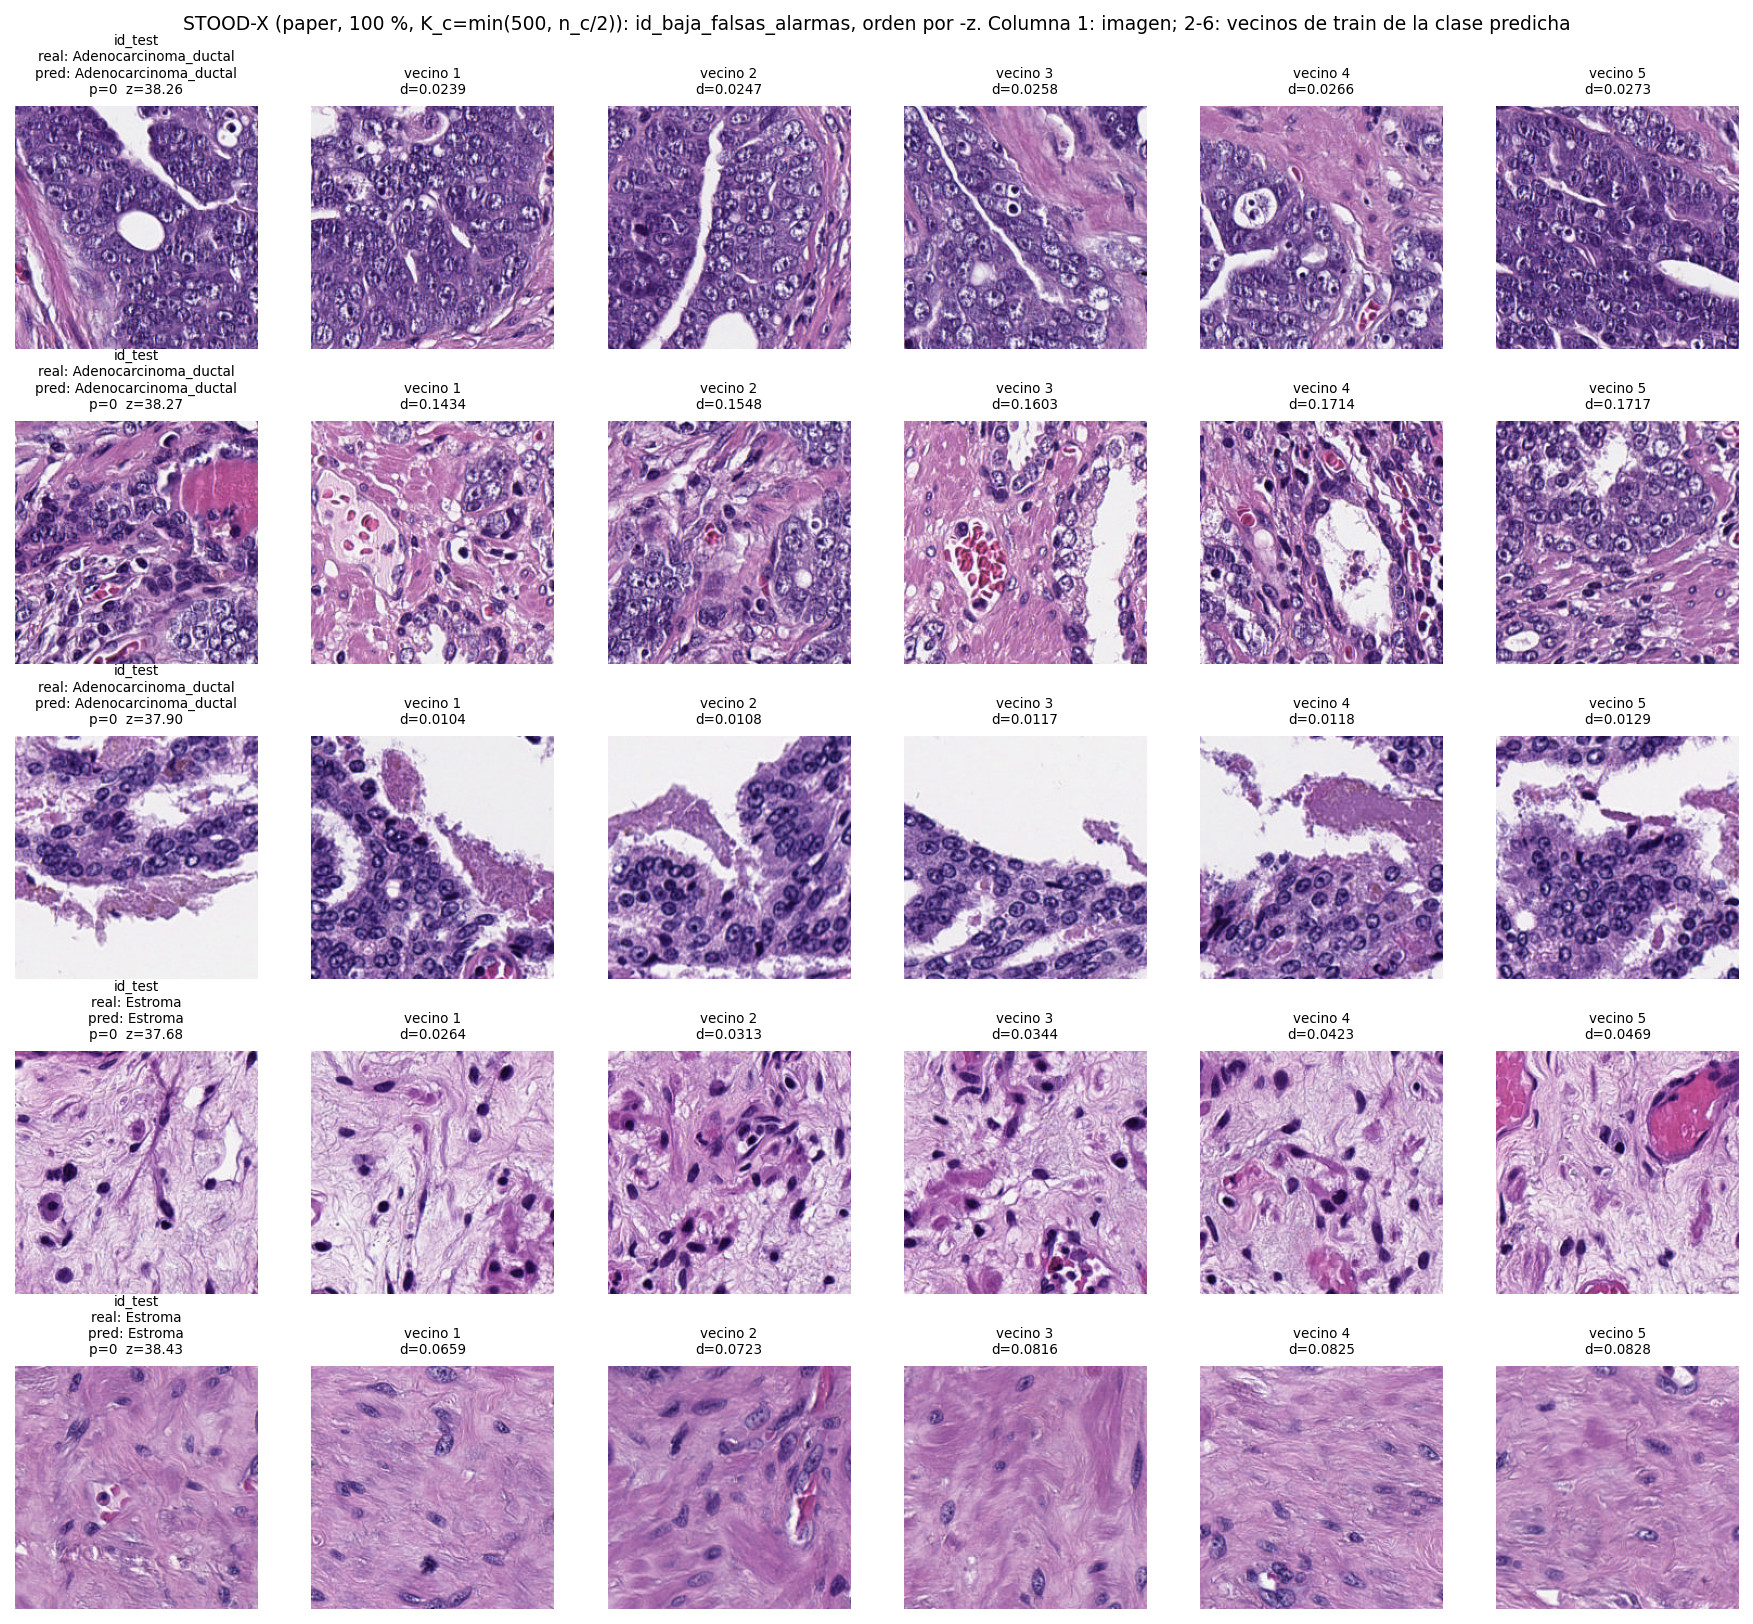
\includegraphics[width=\textwidth]{img/apC/ejemplos_kc_id_baja_falsas_alarmas.jpg}
  \caption{STOOD-X (variante exploratoria $K_c$): cinco imágenes ID con puntuación baja (falsas alarmas) y sus vecinos de entrenamiento de la clase predicha.}
  \label{fig:stoodx-kc-id-falsas}
\end{figure}

\begin{figure}[tbp]
  \centering
  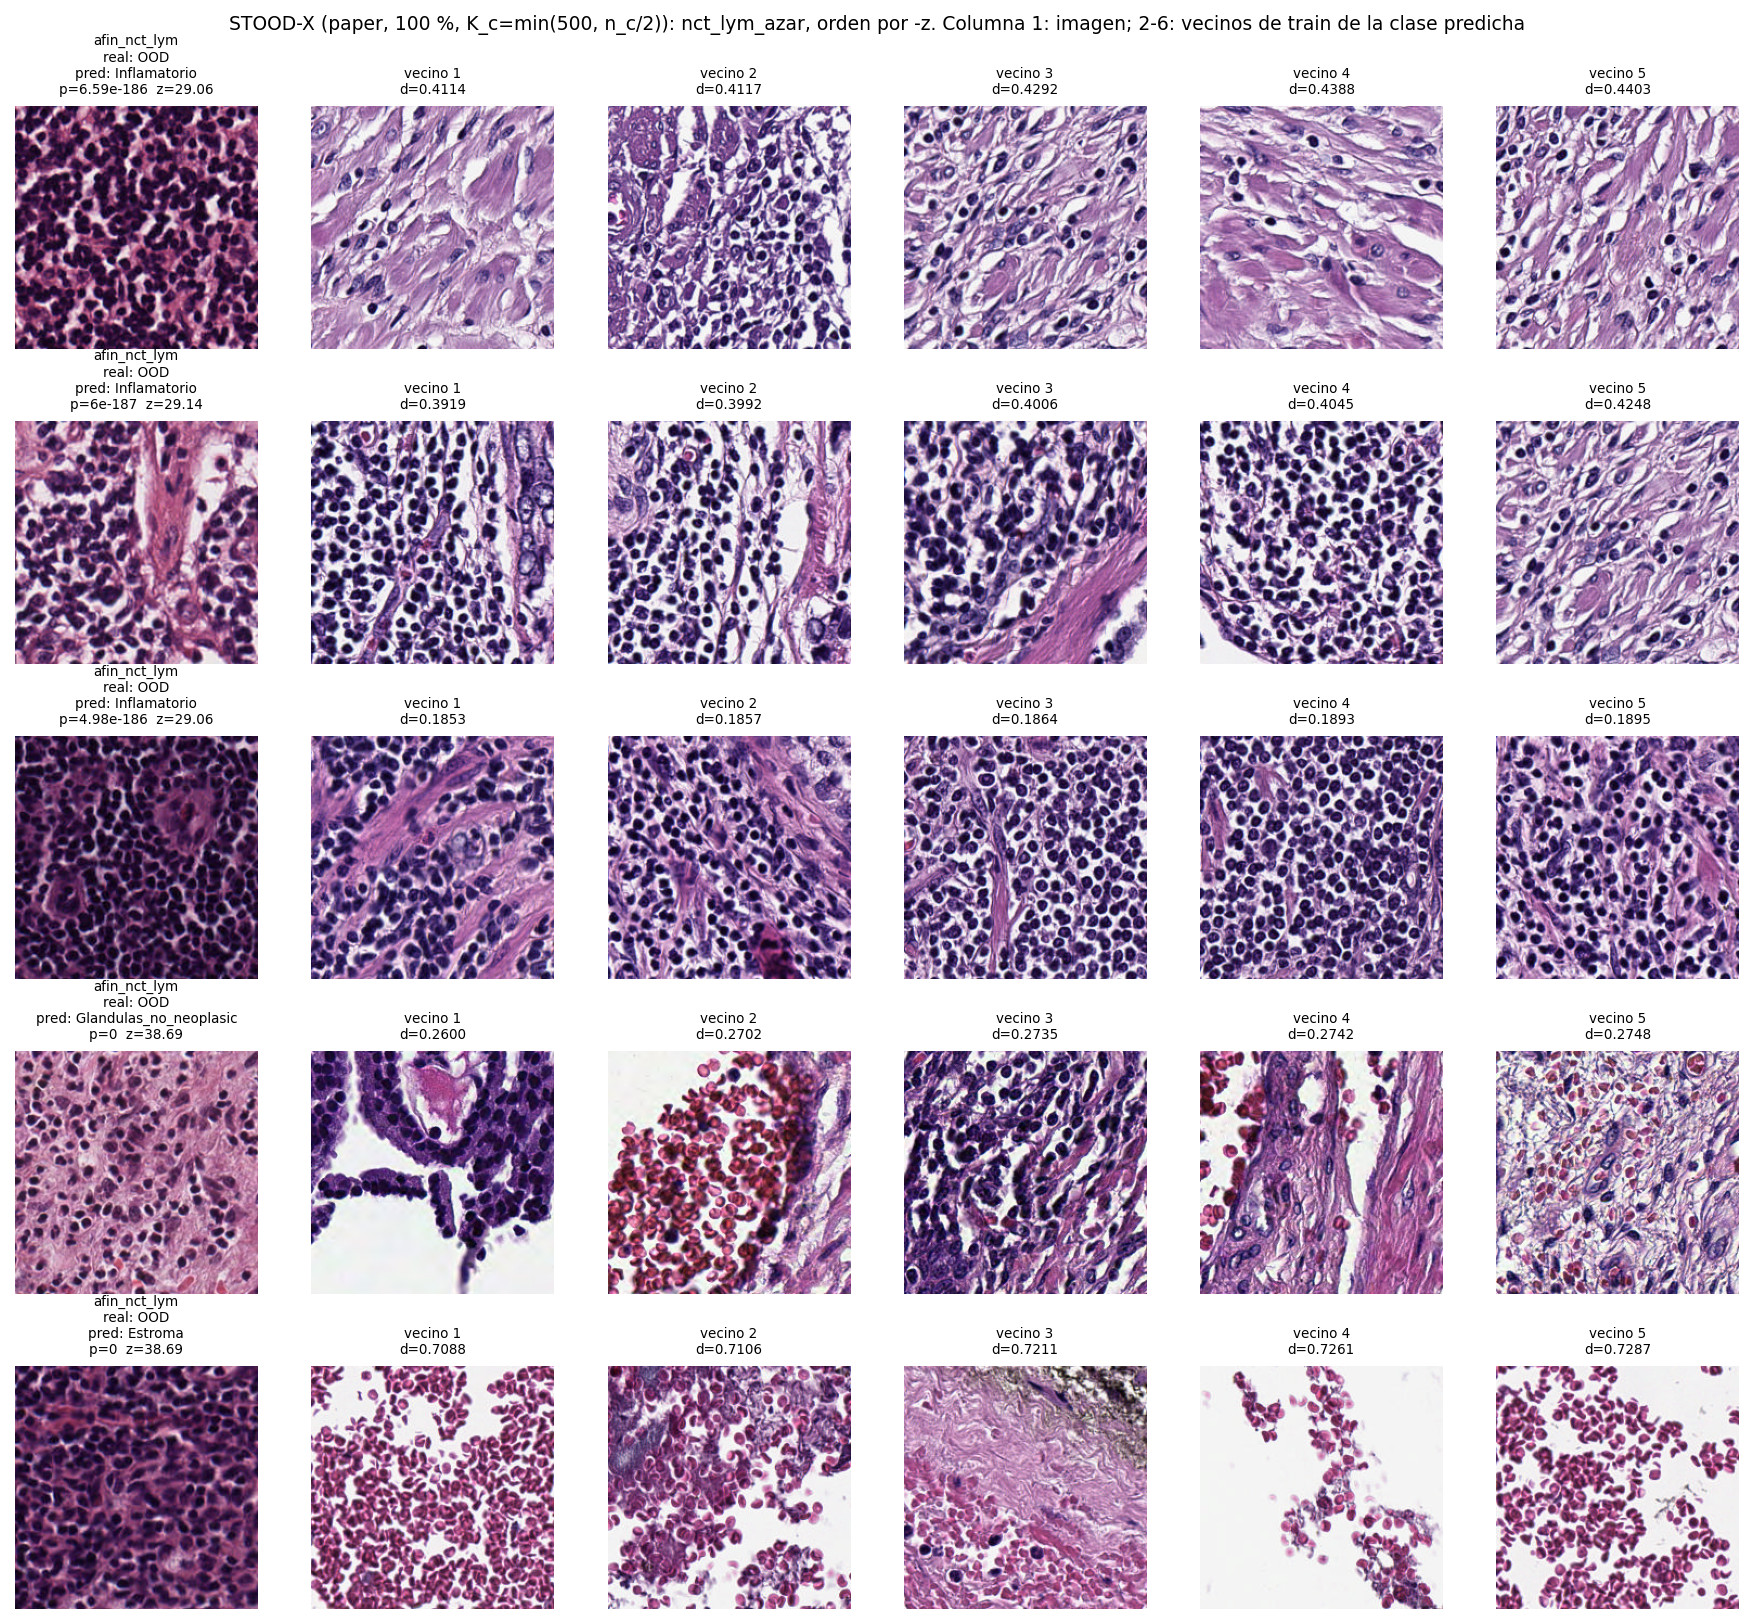
\includegraphics[width=\textwidth]{img/apC/ejemplos_kc_nct_lym_azar.jpg}
  \caption{STOOD-X (variante exploratoria $K_c$): cinco imágenes de LYM elegidas al azar y sus vecinos de entrenamiento de la clase predicha.}
  \label{fig:stoodx-kc-lym}
\end{figure}

\begin{figure}[tbp]
  \centering
  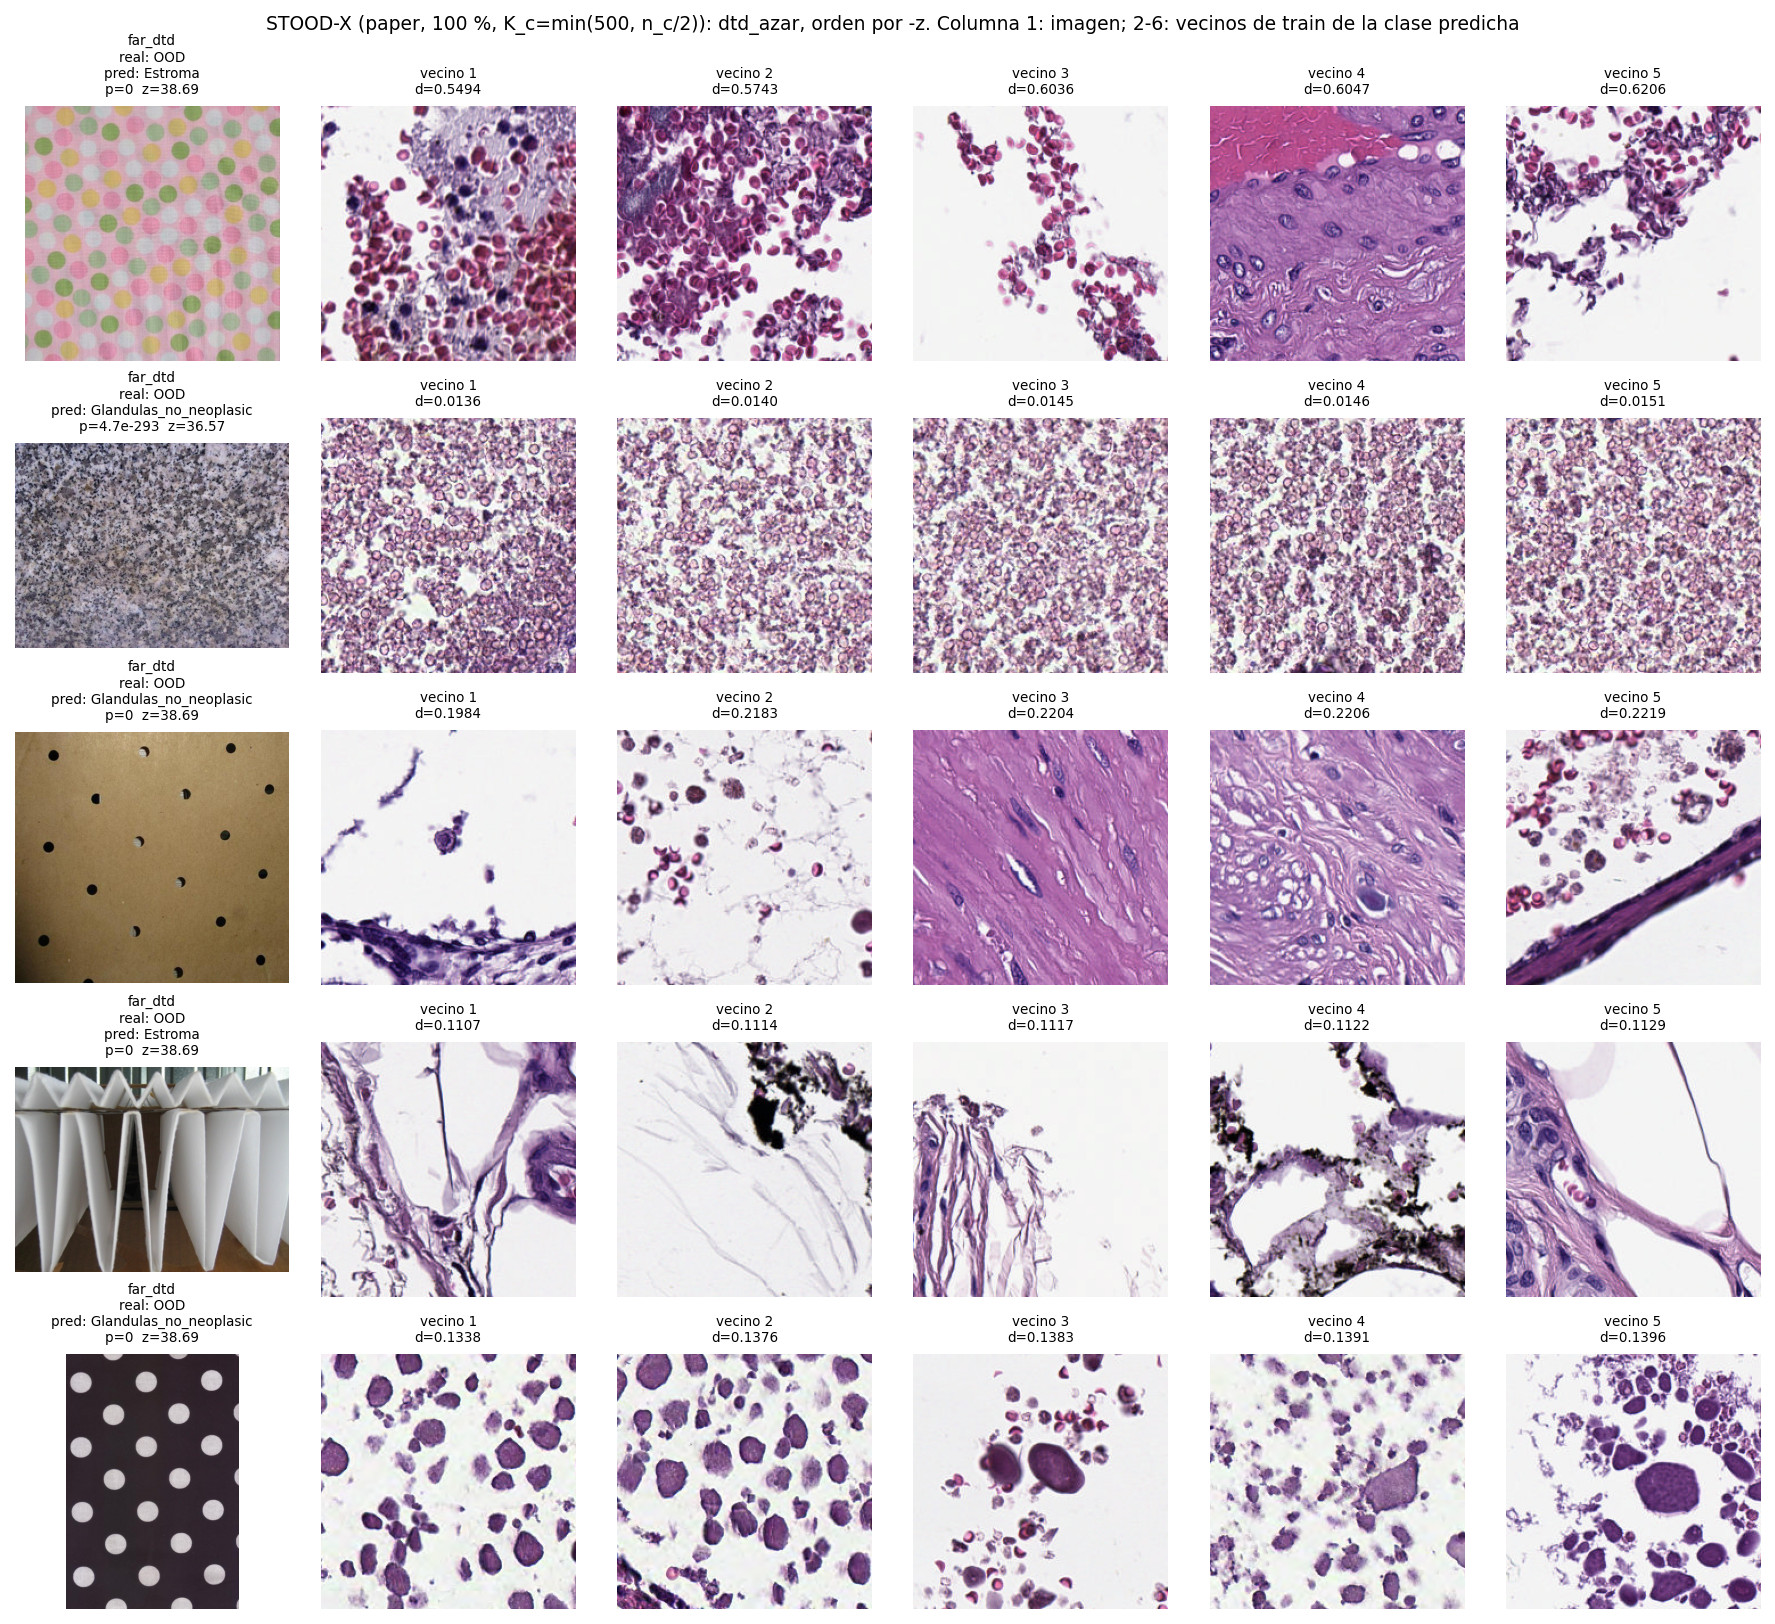
\includegraphics[width=\textwidth]{img/apC/ejemplos_kc_dtd_azar.jpg}
  \caption{STOOD-X (variante exploratoria $K_c$): cinco imágenes de DTD elegidas al azar y sus vecinos de entrenamiento de la clase predicha.}
  \label{fig:stoodx-kc-dtd}
\end{figure}

\clearpage
\section{Imágenes de muestra}\label{sec:apc-muestras}

% Copiadas de tfg/TrainTest/test. Primera imagen: la primera por nombre de fichero (orden de bytes):
% Adenocarcinoma_ductal: 1449748_023745_027329_000224.png
% Carcinoma_intraductal: 1449670_007617_045697_000224.png
% Estroma: 1284741_033377_005153_000224.png
% Glandulas_no_neoplasicas: 1284741_008065_072801_000224.png
% Gleason_3: 12897_011201_018145_000224.png
% Gleason_4_cribiformes: 1284759_012545_016801_000224.png
% Gleason_4_fusionadas: 12903_003361_029121_000224.png
% Gleason_4_glomeruloide: 12903_015905_010977_000224.png
% Gleason_4_pobremente_formadas: 12903_004257_023073_000224.png
% Gleason_5_comedonecrosis: 1449712_010753_064513_000224.png
% Gleason_5_no_glandulas: 1284741_001793_074369_000224.png
% Inflamatorio: 1284753_020385_022177_000224.png
% No_Cancer: 1284741_036289_009185_000224.png
% PIN_de_alto_grado: 12940_018593_064065_000224.png
% Imagen al azar: random.Random(0).choice sobre los ficheros ordenados, con las clases por orden alfabético:
% Adenocarcinoma_ductal: 1570882_012769_071681_000224.png
% Carcinoma_intraductal: 30112282_009633_008961_000224.png
% Estroma: 1449762_032705_012769_000224.png
% Glandulas_no_neoplasicas: 12897_012321_021281_000224.png
% Gleason_3: 12940_023521_057793_000224.png
% Gleason_4_cribiformes: 30112807_006273_017025_000224.png
% Gleason_4_fusionadas: 30113155_031585_029569_000224.png
% Gleason_4_glomeruloide: 1449700_028897_021281_000224.png
% Gleason_4_pobremente_formadas: 1796901_021729_020833_000224.png
% Gleason_5_comedonecrosis: 28890002_025537_026881_000224.png
% Gleason_5_no_glandulas: 1449762_025537_012545_000224.png
% Inflamatorio: 28890002_024417_012321_000224.png
% No_Cancer: 13044_004705_031585_000224.png
% PIN_de_alto_grado: 30121643_008289_019489_000224.png

\begin{figure}[H]
  \centering
  \begin{subfigure}[t]{0.45\textwidth}
    \centering
    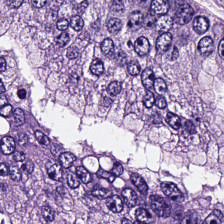
\includegraphics[width=0.095\textheight]{img/apC/muestra_primera_Adenocarcinoma_ductal.png}
    \caption{\clase{Adenocarcinoma\_ductal}}
  \end{subfigure}%
  \begin{subfigure}[t]{0.45\textwidth}
    \centering
    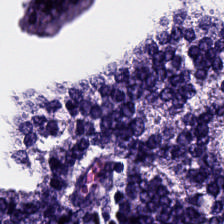
\includegraphics[width=0.095\textheight]{img/apC/muestra_primera_Carcinoma_intraductal.png}
    \caption{\clase{Carcinoma\_intraductal}}
  \end{subfigure}

  \begin{subfigure}[t]{0.45\textwidth}
    \centering
    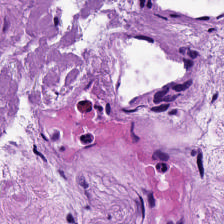
\includegraphics[width=0.095\textheight]{img/apC/muestra_primera_Estroma.png}
    \caption{\clase{Estroma}}
  \end{subfigure}%
  \begin{subfigure}[t]{0.45\textwidth}
    \centering
    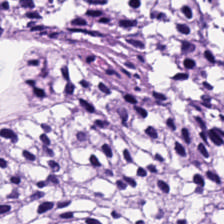
\includegraphics[width=0.095\textheight]{img/apC/muestra_primera_Glandulas_no_neoplasicas.png}
    \caption{\clase{Glandulas\_no\_neoplasicas}}
  \end{subfigure}

  \begin{subfigure}[t]{0.45\textwidth}
    \centering
    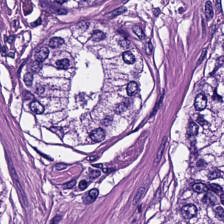
\includegraphics[width=0.095\textheight]{img/apC/muestra_primera_Gleason_3.png}
    \caption{\clase{Gleason\_3}}
  \end{subfigure}%
  \begin{subfigure}[t]{0.45\textwidth}
    \centering
    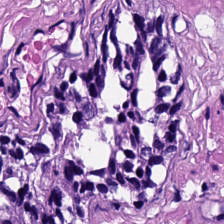
\includegraphics[width=0.095\textheight]{img/apC/muestra_primera_Gleason_4_cribiformes.png}
    \caption{\clase{Gleason\_4\_cribiformes}}
  \end{subfigure}

  \begin{subfigure}[t]{0.45\textwidth}
    \centering
    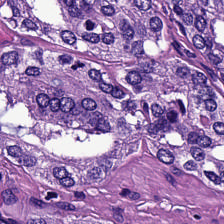
\includegraphics[width=0.095\textheight]{img/apC/muestra_primera_Gleason_4_fusionadas.png}
    \caption{\clase{Gleason\_4\_fusionadas}}
  \end{subfigure}%
  \begin{subfigure}[t]{0.45\textwidth}
    \centering
    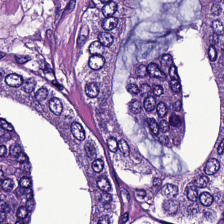
\includegraphics[width=0.095\textheight]{img/apC/muestra_primera_Gleason_4_glomeruloide.png}
    \caption{\clase{Gleason\_4\_glomeruloide}}
  \end{subfigure}

  \begin{subfigure}[t]{0.45\textwidth}
    \centering
    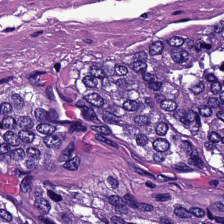
\includegraphics[width=0.095\textheight]{img/apC/muestra_primera_Gleason_4_pobremente_formadas.png}
    \caption{\clase{Gleason\_4\_pobremente\_formadas}}
  \end{subfigure}%
  \begin{subfigure}[t]{0.45\textwidth}
    \centering
    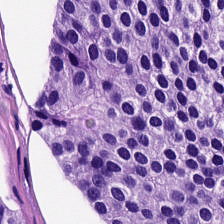
\includegraphics[width=0.095\textheight]{img/apC/muestra_primera_Gleason_5_comedonecrosis.png}
    \caption{\clase{Gleason\_5\_comedonecrosis}}
  \end{subfigure}

  \begin{subfigure}[t]{0.45\textwidth}
    \centering
    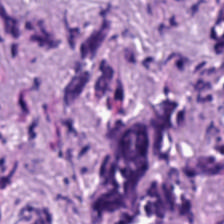
\includegraphics[width=0.095\textheight]{img/apC/muestra_primera_Gleason_5_no_glandulas.png}
    \caption{\clase{Gleason\_5\_no\_glandulas}}
  \end{subfigure}%
  \begin{subfigure}[t]{0.45\textwidth}
    \centering
    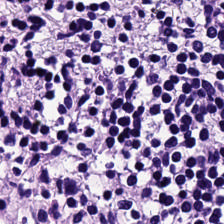
\includegraphics[width=0.095\textheight]{img/apC/muestra_primera_Inflamatorio.png}
    \caption{\clase{Inflamatorio}}
  \end{subfigure}

  \begin{subfigure}[t]{0.45\textwidth}
    \centering
    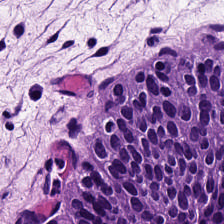
\includegraphics[width=0.095\textheight]{img/apC/muestra_primera_No_Cancer.png}
    \caption{\clase{No\_Cancer}}
  \end{subfigure}%
  \begin{subfigure}[t]{0.45\textwidth}
    \centering
    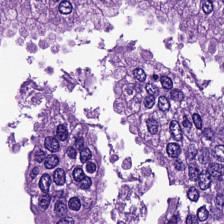
\includegraphics[width=0.095\textheight]{img/apC/muestra_primera_PIN_de_alto_grado.png}
    \caption{\clase{PIN\_de\_alto\_grado}}
  \end{subfigure}
  \caption{Primera imagen de cada clase del conjunto de test, por orden de nombre de fichero. \revisar{pie de figura redactado por el agente}}
  \label{fig:muestras-primera}
\end{figure}

\begin{figure}[H]
  \centering
  \begin{subfigure}[t]{0.45\textwidth}
    \centering
    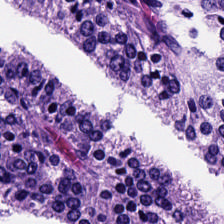
\includegraphics[width=0.095\textheight]{img/apC/muestra_azar_Adenocarcinoma_ductal.png}
    \caption{\clase{Adenocarcinoma\_ductal}}
  \end{subfigure}%
  \begin{subfigure}[t]{0.45\textwidth}
    \centering
    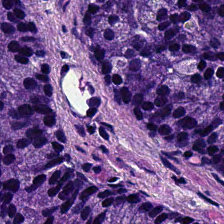
\includegraphics[width=0.095\textheight]{img/apC/muestra_azar_Carcinoma_intraductal.png}
    \caption{\clase{Carcinoma\_intraductal}}
  \end{subfigure}

  \begin{subfigure}[t]{0.45\textwidth}
    \centering
    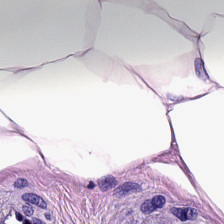
\includegraphics[width=0.095\textheight]{img/apC/muestra_azar_Estroma.png}
    \caption{\clase{Estroma}}
  \end{subfigure}%
  \begin{subfigure}[t]{0.45\textwidth}
    \centering
    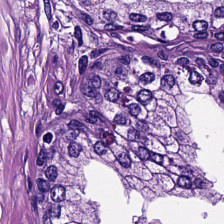
\includegraphics[width=0.095\textheight]{img/apC/muestra_azar_Glandulas_no_neoplasicas.png}
    \caption{\clase{Glandulas\_no\_neoplasicas}}
  \end{subfigure}

  \begin{subfigure}[t]{0.45\textwidth}
    \centering
    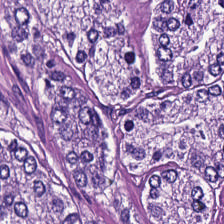
\includegraphics[width=0.095\textheight]{img/apC/muestra_azar_Gleason_3.png}
    \caption{\clase{Gleason\_3}}
  \end{subfigure}%
  \begin{subfigure}[t]{0.45\textwidth}
    \centering
    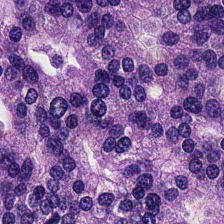
\includegraphics[width=0.095\textheight]{img/apC/muestra_azar_Gleason_4_cribiformes.png}
    \caption{\clase{Gleason\_4\_cribiformes}}
  \end{subfigure}

  \begin{subfigure}[t]{0.45\textwidth}
    \centering
    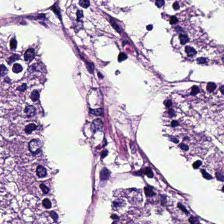
\includegraphics[width=0.095\textheight]{img/apC/muestra_azar_Gleason_4_fusionadas.png}
    \caption{\clase{Gleason\_4\_fusionadas}}
  \end{subfigure}%
  \begin{subfigure}[t]{0.45\textwidth}
    \centering
    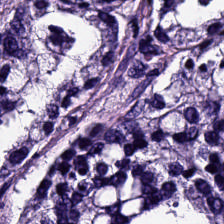
\includegraphics[width=0.095\textheight]{img/apC/muestra_azar_Gleason_4_glomeruloide.png}
    \caption{\clase{Gleason\_4\_glomeruloide}}
  \end{subfigure}

  \begin{subfigure}[t]{0.45\textwidth}
    \centering
    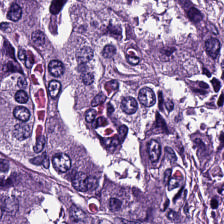
\includegraphics[width=0.095\textheight]{img/apC/muestra_azar_Gleason_4_pobremente_formadas.png}
    \caption{\clase{Gleason\_4\_pobremente\_formadas}}
  \end{subfigure}%
  \begin{subfigure}[t]{0.45\textwidth}
    \centering
    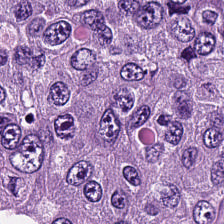
\includegraphics[width=0.095\textheight]{img/apC/muestra_azar_Gleason_5_comedonecrosis.png}
    \caption{\clase{Gleason\_5\_comedonecrosis}}
  \end{subfigure}

  \begin{subfigure}[t]{0.45\textwidth}
    \centering
    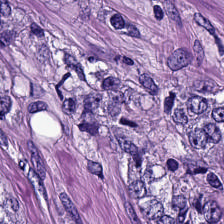
\includegraphics[width=0.095\textheight]{img/apC/muestra_azar_Gleason_5_no_glandulas.png}
    \caption{\clase{Gleason\_5\_no\_glandulas}}
  \end{subfigure}%
  \begin{subfigure}[t]{0.45\textwidth}
    \centering
    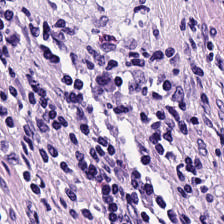
\includegraphics[width=0.095\textheight]{img/apC/muestra_azar_Inflamatorio.png}
    \caption{\clase{Inflamatorio}}
  \end{subfigure}

  \begin{subfigure}[t]{0.45\textwidth}
    \centering
    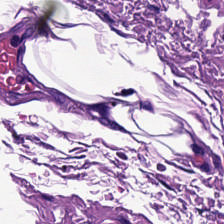
\includegraphics[width=0.095\textheight]{img/apC/muestra_azar_No_Cancer.png}
    \caption{\clase{No\_Cancer}}
  \end{subfigure}%
  \begin{subfigure}[t]{0.45\textwidth}
    \centering
    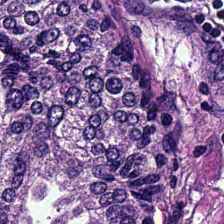
\includegraphics[width=0.095\textheight]{img/apC/muestra_azar_PIN_de_alto_grado.png}
    \caption{\clase{PIN\_de\_alto\_grado}}
  \end{subfigure}
  \caption{Una imagen elegida al azar de cada clase del conjunto de test. \revisar{pie de figura redactado por el agente}}
  \label{fig:muestras-azar}
\end{figure}

% Otro posible material complementario (decidir):
% - Variantes de las agrupaciones clínicas (opción b ISUP y PIN no maligno; results_agrupaciones).
% - Histogramas de puntuaciones por método y conjunto (fig3_histogramas de la fase C).
% - Configuración completa de los experimentos.

\endinput
